\documentclass[11pt]{article}
\usepackage[margin=0.85in]{geometry}
\usepackage{amsmath,graphicx,booktabs,longtable,float,xcolor,caption,subcaption}
\usepackage[authoryear,round]{natbib}
\usepackage[colorlinks=true,linkcolor=blue,urlcolor=blue,citecolor=blue]{hyperref}
\setlength{\parindent}{0pt}\setlength{\parskip}{6pt}
\renewcommand{\thefigure}{R\arabic{figure}}
\title{Independent reconstruction of regional climate-informed West Nile neuroinvasive disease forecasts}
\author{Reproducible research implementation for Raul Moreno}
\date{8 October 2026}
\begin{document}\maketitle
\begin{abstract}
We implement the regional negative-binomial Bayesian regression and retrospective
evaluation described by Harp et al. (2026), using independently acquired public
county disease counts and gridded climate inputs. We reconstruct county and regional
case summaries, climate correlations, probabilistic forecasts, and score uncertainty.
The executed analysis is incomplete: NASA NLDAS soil moisture required by several
published predictor sets returned HTTP 401. We therefore distinguish exact published
predictor fits where inputs are available from an explicitly restricted-candidate
analysis using PRISM and gridMET. Synthetic recovery, independent MCMC, predictive
checks, and scoring identities test the implementation. No original author code,
deposited data, submitted competition forecast, or digitized plot enters the analysis.
\end{abstract}
\section{Scope and evidence}
The target is \citet{harp}, GeoHealth 10(2), e2025GH001657. Written Sections 2.1--2.6,
Tables 1--2, and Supporting Information S1 provide the specification. All plotted
numbers in this report were calculated by this implementation from public inputs.
No published image appears in the report. Reproduced means that we generated the
specified quantity independently; it does not imply numerical identity with the
publication. Input vintages and explicit interpretation choices remain material.
Descriptive case maps and correlation maps are identified separately from model
forecasts. The study-region locator is a schematic and is not a reproduced model result.
Report figures carry an R prefix; source-paper figure identifiers are stated in
their captions and in the panel registry.
Independently reproduced panels: 1a, 1b, 1c, 1d, 2a, 2b, 2c, 2d, 3a, 3b, 3c, 3d, S13, S16, S17, S18, S20. Partially reproduced panels: 4, 5, S1, S2, S3, S4, S5, S6, S7, S8, S9, S10, S11, S12, S14, S15, S19, S21, S22, S23, S24. The competition comparisons and county mixed-model extension are not reproduced.
\section{Inputs and spatial processing}
CDC's public ArboNET dashboard supplies annual county WNND counts. We use its
historical release finalized 16 September 2026 and subset 2005--2022. A separate
CDC file supplies 2022 Connecticut counties, whose rows in the main file are
unavailable planning-region placeholders. Missing county-year activity rows are
interpreted as zero reported cases; explicit missing case values are rejected.
Legacy Shannon/Oglala Lakota and Bedford identifiers are harmonized to Census 2020
boundaries. Alaska, Hawaii, and territories are excluded. County totals match
independently downloaded contiguous-state totals in 17 of 18 years. Two Iowa cases
in 2010 use unknown county code 19999; we retain this documented discrepancy
rather than assign cases to a region without evidence.

Counties are assigned to NEON October 2024 polygons using Census 2020 population
centers. Coastal centers outside a polygon use the nearest polygon in EPSG:5070;
the exception log gives all distances. We use 2020 cartographic county polygons at
1:500,000. Each county climate mean weights grid cells by cosine latitude, including
cells whose centers lie inside the original polygon. Counties without valid cell
centers use the nearest valid cell at their population center. This approximates
fractional-cell integration; display geometries alone are simplified. Domain maps
are clipped to the continental viewing window to omit noncontinental fragments.

The paper's text selects regions with at least 1,000 historical cases, whereas
Figure 1's caption describes a 50-case annual-mean threshold. Current inputs give
Mid Atlantic 987 cases; we retain the 11 explicitly named regions to preserve the
comparison. These 11 regions contain 92.7 percent of the independently assigned
continental county cases, compared with the paper's statement of more than
93 percent. Regional climate weights are $w_c=\log H_c$, where $H_c$ is each county's
total 2005--2022 cases. Counties with $H_c=0$ are excluded and $H_c=1$ has zero weight.
The regional covariate is $x_{rt}=\sum_{c\in r}w_c x_{ct}/\sum_{c\in r}w_c$.

We download 720 PRISM monthly grids from the NC State Climate Office's public
THREDDS service, with Oregon State PRISM identified in their metadata. Variables
are mean temperature, mean dew point (${}^\circ\mathrm{C}$), precipitation
($\mathrm{mm}$ per month), and maximum vapor pressure deficit ($\mathrm{hPa}$).
The seasonal window is previous October--December and concurrent January--July.
These contemporary reprocessed inputs need not equal the paper's 2023 input vintage.
gridMET pentad PDSI is averaged by calendar month before county reduction; the
accessible metadata describe a 1980--2019 reference period. The paper does not
specify how pentads were reduced to months.

NLDAS soil moisture could not be downloaded anonymously (HTTP 401); its legacy
GrADS endpoint returned HTTP 410. The paper does not identify the land-surface
model or version. A proposed, unexecuted interpretation is Noah monthly v2.0,
0--100 mm layer moisture, whose midpoint is 50 mm. No alternate soil product is
substituted here. Our explicit missing soil row limits the six-variable screening
and any model requiring soil moisture. Data versions, URL hashes, access times,
transformations, and failed attempts are recorded in the repository's provenance
files. Large raw downloads are excluded from Git and downloadable by script.
\begin{figure}[H]\centering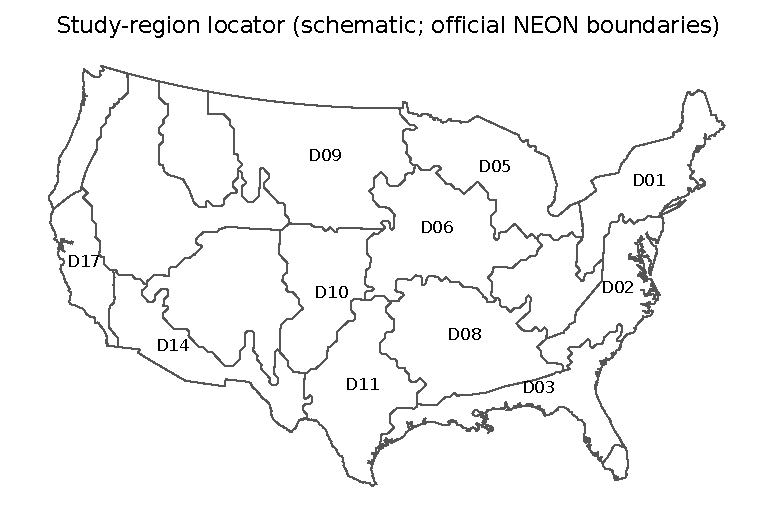
\includegraphics[width=\textwidth]{../figures/region_schematic.pdf}\caption{Study-region locator, redrawn from official NEON polygons. Labels identify the 11 modeled domains; unlabelled domains are excluded. This is a schematic, not a numerical reproduction.}\end{figure}
\section{Regression and retrospective evaluation}
For each region and year, we model the raw count $Y_t$ by
\begin{equation}
Y_t\mid\mu_t,\phi\sim\mathrm{NB2}(\mu_t,\phi),\qquad
\log\mu_t=\alpha+\sum_j\beta_j z_{tj},\qquad
\mathrm{Var}(Y_t)=\mu_t+\mu_t^2/\phi.
\end{equation}
Here $z$ is the climate predictor centered and scaled by the training fold's mean
and sample standard deviation. The univariable and bivariable models have one and
two climate predictors. The historical benchmark has an intercept alone, with
the same dispersion and prior treatment. All models are independent across regions.
The supplement writes a linear expression for the mean but names
\texttt{stan\_glm.nb}, whose default link is logarithmic. We interpret the displayed
linear expression as the linear predictor and use the log link. Counts are not
logged before fitting the count likelihood.

We infer numerical prior settings from the official rstanarm defaults
\citep{rstanarm}: independent $\alpha,\beta_j\sim N(0,2.5^2)$ on the centered,
standardized scale and $\phi\sim\mathrm{Exponential}(1)$. These are weakly informative,
not flat priors. The written supplement does not enumerate numerical prior scales.
Our sampler includes the Jacobian for $\log\phi$. It uses a 7-degree-of-freedom
multivariate Student proposal centered at the posterior mode, found with an
analytic gradient, with scale 1.2 times the inverse finite-difference Hessian.
Exact posterior-to-proposal weights correct
the proposal. Thus a Gaussian curvature calculation does not replace the posterior.
Four independent batches begin with 8,192 proposals each; sample sizes double if
importance effective sample size is below 4,000 or Pareto $k\geq0.7$. Numerical pass
also requires mean Monte Carlo error below 0.05 posterior standard deviations.
This replaces the paper's four Stan chains of 500 warmup and 500 retained draws.
Independent Metropolis chains test the numerical substitution.

Predictor selection ranks absolute Pearson correlations between $\log Y_t$ and
the 60 potential month-variable combinations. Secondary variables must come from
a different group: air conditions (temperature, dew point, VPD), antecedent soil
conditions (PDSI, soil moisture), or precipitation. The executed restricted analysis
screens 50 available candidates, then uses the same two-group constraint. We also
fit the exact Table 1 predictor sets when their inputs are present. Screening and
county climate weights use the full 18-year record, as described in the paper.
They are not recomputed inside each validation fold; this can favor retrospective
skill and precludes interpreting these scores as a prospective validation.

Each held-out year is predicted from a fit to the other 17 years. Thus early years
are predicted using later observations. We generate 30,000 posterior predictive
integer draws and save 23 empirical quantiles at 1, 2.5, 5, 10, 15,\ldots,95,97.5,
and 99 percent. Seeds, parameter summaries, fold predictions, and diagnostics are
saved. The full-model input pathway supports soil moisture when independent raw
files become available, but those results are absent from this run.

\subsection{Skill and uncertainty}
We apply $\log(1+x)$ to observed counts and forecast quantiles. For $K=11$ central
intervals with lower and upper bounds $l_k,u_k$ and miscoverage $a_k$, the score is
\begin{align}
\mathrm{IS}_{a_k}&=(u_k-l_k)+\frac{2}{a_k}(l_k-y)\mathbf{1}_{y<l_k}
 +\frac{2}{a_k}(y-u_k)\mathbf{1}_{y>u_k},\\
\mathrm{WIS}&=\frac{\frac12|y-m|+\sum_{k=1}^{11}\frac{a_k}{2}\mathrm{IS}_{a_k}}{11.5}.
\end{align}
The median is $m$; the three components are width, overprediction, and
underprediction \citep{bracher}. We allocate the median term to the appropriate
signed component, so the components sum exactly. Lower WIS is better.
Percent improvement is $100(\mathrm{WIS}_{B}-\mathrm{WIS}_{M})/\mathrm{WIS}_{B}$.

Regional uncertainty uses 10,000 paired resamples of 18 years. National scores
weight regional scores by historical cases. National uncertainty resamples both
regions and years and renormalizes those weights; this is an explicit interpretation
of incompletely specified bootstrap details. Year draws are paired between models
but independent between regions, so synchronous regional shocks are not preserved;
this choice can affect national interval widths. The national score is not the score
of a national total-count forecast. Intervals are bootstrap 2.5th and 97.5th
percentiles. PIT uses the midpoint of the predictive CDF jump at an integer
observation; interval coverage includes endpoints.
\section{Numerical results and comparison}
The restricted-candidate univariable model gives a national median improvement of 15.4\% (4.6 to 25.5\%), compared with the published 18.8\% (4.7 to 27.7\%). The difference is -3.4 percentage points. These estimates compare different predictor-selection spaces because soil moisture is missing.

The restricted-candidate bivariable model gives a national median improvement of 18.7\% (5.6 to 30.3\%), compared with the published 21.8\% (7.0 to 30.7\%). The difference is -3.1 percentage points. These estimates compare different predictor-selection spaces because soil moisture is missing.

As a benchmark sanity check, the independent regional mean historical-model WIS differs from the rounded published values in Supplementary Table S5 by a mean absolute 0.004 and a maximum absolute 0.010. The full regional comparison is saved in benchmark\_comparison.csv. This check isolates the disease data and count-distribution model from the missing climate input.
\begin{table}[H]\centering\small\begin{tabular}{lrrrr}\toprule Region & Paper uni (\%) & Ours uni (\%) & Paper bi (\%) & Ours bi (\%)\\\midrule
Pacific Southwest & 25.3 & 24.6 & 20.8 & 17.6 \\
Desert Southwest & 11.3 & 10.7 & 7.2 & 3.0 \\
Northern Plains & 33.4 & 31.3 & 52.6 & 51.9 \\
Central Plains & 1.9 & 1.8 & 25.7 & 25.1 \\
Southern Plains & 32.9 & 10.0 & 31.6 & 19.0 \\
Prairie Peninsula & 29.5 & 22.5 & 33.5 & 21.9 \\
Ozarks Complex & 29.5 & 30.1 & 35.2 & 34.4 \\
Great Lakes & 10.7 & 12.4 & 10.5 & 8.3 \\
Southeast & 10.1 & 6.5 & 13.0 & 9.6 \\
Mid Atlantic & 17.6 & 17.8 & 32.3 & 35.2 \\
Northeast & 5.2 & 2.9 & 7.9 & 0.2 \\
National & 18.8 & 15.4 & 21.8 & 18.7 \\
\bottomrule\end{tabular}\caption{Published Table 2 medians versus independent restricted-candidate screening. Published numbers are transcribed text references and do not enter fitting or generated plots. Full intervals and differences are saved in results/published\_comparison.csv.}\end{table}
\begin{table}[H]\centering\small\begin{tabular}{llrr}\toprule Region & Published predictor model & Paper (\%) & Independent median [95\% interval]\\\midrule
Pacific Southwest & uni & 25.3 & 24.9 [-0.4, 42.2] \\
Desert Southwest & uni & 11.3 & 9.9 [-9.9, 25.9] \\
Desert Southwest & bi & 7.2 & 7.1 [-22.9, 27.0] \\
Northern Plains & uni & 33.4 & 30.8 [10.0, 46.4] \\
Northern Plains & bi & 52.6 & 52.0 [33.8, 63.3] \\
Central Plains & uni & 1.9 & 1.9 [-12.8, 10.6] \\
Central Plains & bi & 25.7 & 24.9 [-2.2, 42.1] \\
Ozarks Complex & uni & 29.5 & 30.0 [2.3, 48.1] \\
Ozarks Complex & bi & 35.2 & 34.7 [8.1, 54.4] \\
Mid Atlantic & uni & 17.6 & 18.2 [-6.4, 35.0] \\
Mid Atlantic & bi & 32.3 & 35.7 [8.2, 54.4] \\
\bottomrule\end{tabular}\caption{Separate fits using the exact written Table 1 predictor sets wherever available. Differences can still reflect data vintage, geometry, monthly aggregation, prior interpretation, and numerical integration.}\end{table}
\begin{table}[H]\centering\scriptsize\begin{tabular}{lllll}\toprule Region & Paper primary & Selected primary & Paper secondary & Selected secondary\\\midrule
Pacific Southwest & tmean\_03 & tmean\_03 & soil\_06 & ppt\_07 \\
Desert Southwest & tmean\_07 & vpdmax\_07 & ppt\_07 & ppt\_07 \\
Northern Plains & tmean\_05 & tmean\_05 & pdsi\_03 & pdsi\_03 \\
Central Plains & tdmean\_06 & tdmean\_06 & pdsi\_10 & pdsi\_10 \\
Southern Plains & soil\_10 & ppt\_03 & ppt\_03 & pdsi\_11 \\
Prairie Peninsula & soil\_03 & pdsi\_07 & tmean\_05 & tmean\_05 \\
Ozarks Complex & pdsi\_11 & pdsi\_11 & tdmean\_06 & tdmean\_06 \\
Great Lakes & soil\_03 & tmean\_01 & tmean\_01 & ppt\_12 \\
Southeast & soil\_01 & vpdmax\_05 & vpdmax\_05 & ppt\_10 \\
Mid Atlantic & tmean\_05 & tmean\_05 & ppt\_07 & ppt\_07 \\
Northeast & soil\_12 & tdmean\_10 & tmean\_05 & ppt\_12 \\
\bottomrule\end{tabular}\caption{Predictor names encode variable and calendar month; months 10--12 are previous-year values. Selection uses all years and five available variables. Soil moisture candidates are absent, so equality with published selection is not expected.}\end{table}
Independent screening agrees with 5 of 11 published primary predictors and 6 of 11 secondary predictors. Both match in 4 regions: Northern Plains, Central Plains, Ozarks Complex, Mid Atlantic. In several soil-dependent regions, the available-input screen promotes the published secondary variable; this is a change in model specification rather than evidence that the original soil effect is absent.
\begin{table}[H]\centering\small\begin{tabular}{lrrr}\toprule Region & Table S1 slope & Independent slope & Independent bounds\\\midrule
Pacific Southwest & +0.271 & +0.269 & [+0.099, +0.439] \\
Desert Southwest & -0.928 & -0.928 & [-1.554, -0.302] \\
Northern Plains & -0.447 & +0.552 & [+0.242, +0.884] \\
Central Plains & -0.244 & +0.153 & [-0.110, +0.423] \\
Ozarks Complex & -0.237 & -0.237 & [-0.369, -0.108] \\
Mid Atlantic & +0.327 & +0.334 & [+0.125, +0.543] \\
\bottomrule\end{tabular}\caption{Univariable coefficients using the exact written predictors, in their raw input units. Each entry averages the posterior mean or 95 percent bound over the 18 held-out fits, matching the stated Table S1 summary. These averaged bounds are not a pooled posterior interval.}\end{table}
The Northern Plains temperature and Central Plains dew-point slopes have
opposite signs to the entries printed in Supplementary Table S1. Other obtainable
slopes agree closely in sign and magnitude. Our signs follow the independently
calculated input associations and fitted likelihood. The written descriptions do
not resolve whether the disagreement reflects a table error, an undocumented
transformation, or different inputs. We retain the discrepancy; no sign was changed
to match the reference. All fold-specific coefficients and dispersion estimates
are saved in results/parameters.csv.
\begin{figure}[H]\centering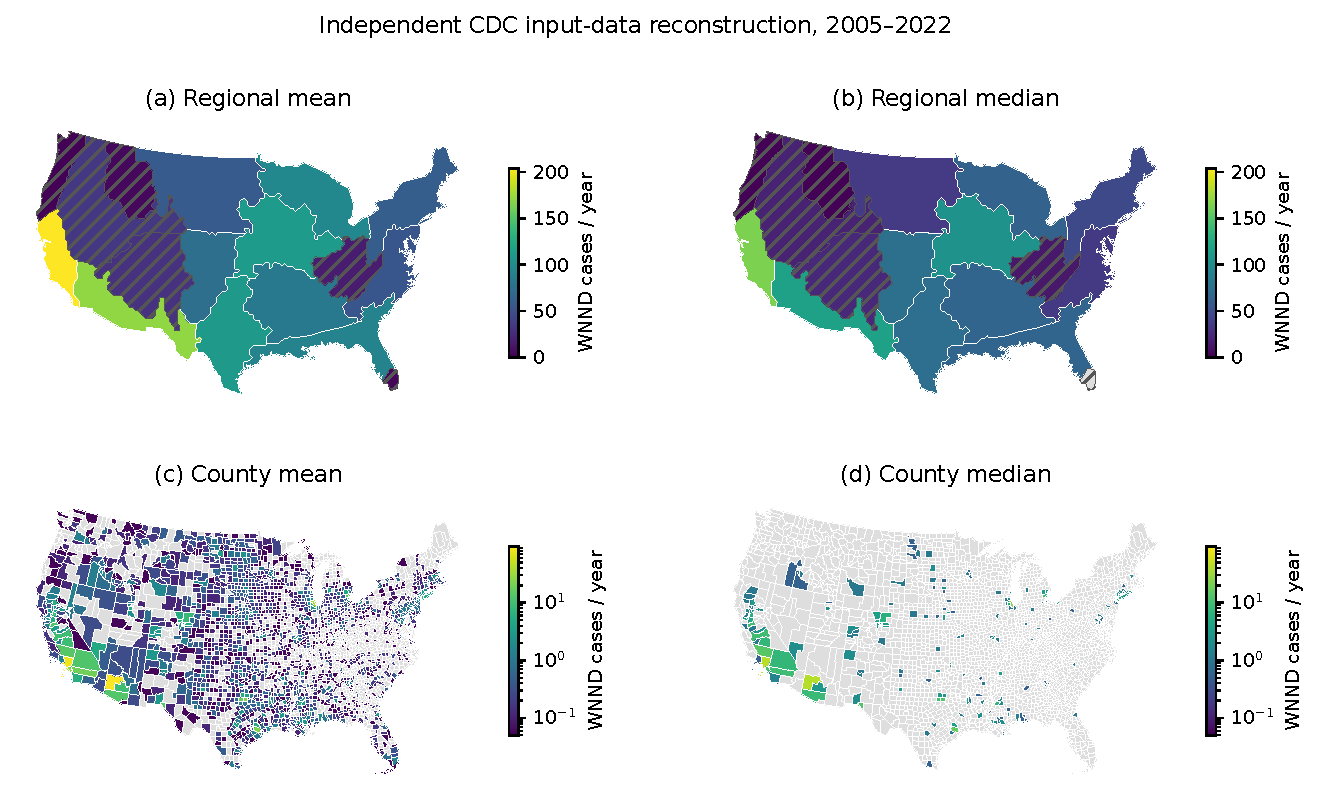
\includegraphics[width=\textwidth]{../figures/figure1.pdf}\caption{Independent Figure 1 reconstruction: (a,b) regional mean and median annual CDC WNND cases; (c,d) corresponding county quantities, 2005--2022. Grey county polygons have zero cases; hatching indicates excluded domains. Regional colors are linear and county colors logarithmic. These are descriptive observational summaries, not fitted model results.}\end{figure}
\begin{figure}[H]\centering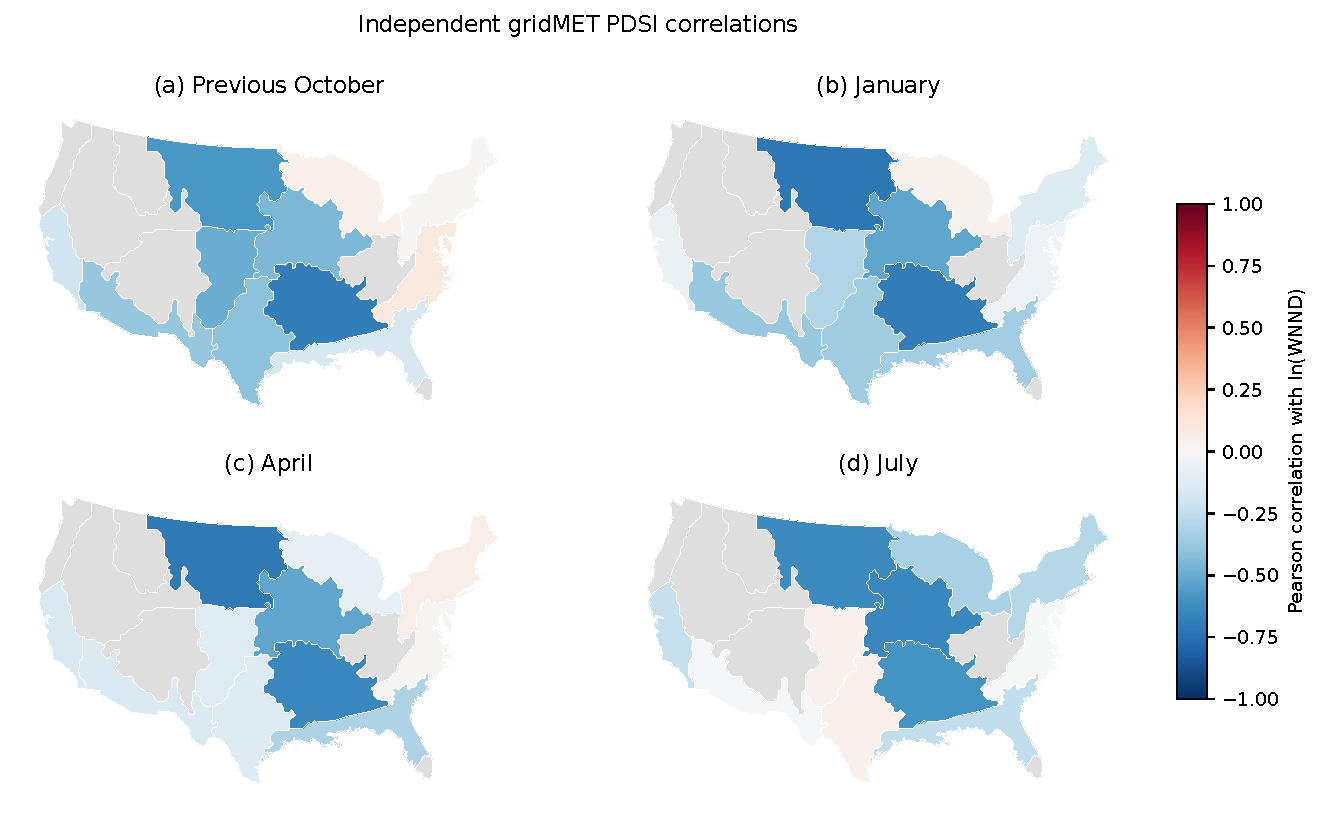
\includegraphics[width=\textwidth]{../figures/figure2.pdf}\caption{Independent Figure 2 reconstruction: correlation between log annual WNND and gridMET PDSI in (a) previous October, (b) January, (c) April, and (d) July. Positive PDSI denotes wetter conditions. Red means positive correlation and blue negative; grey domains are excluded. Each correlation uses 18 years and log-case county weights.}\end{figure}
\begin{figure}[H]\centering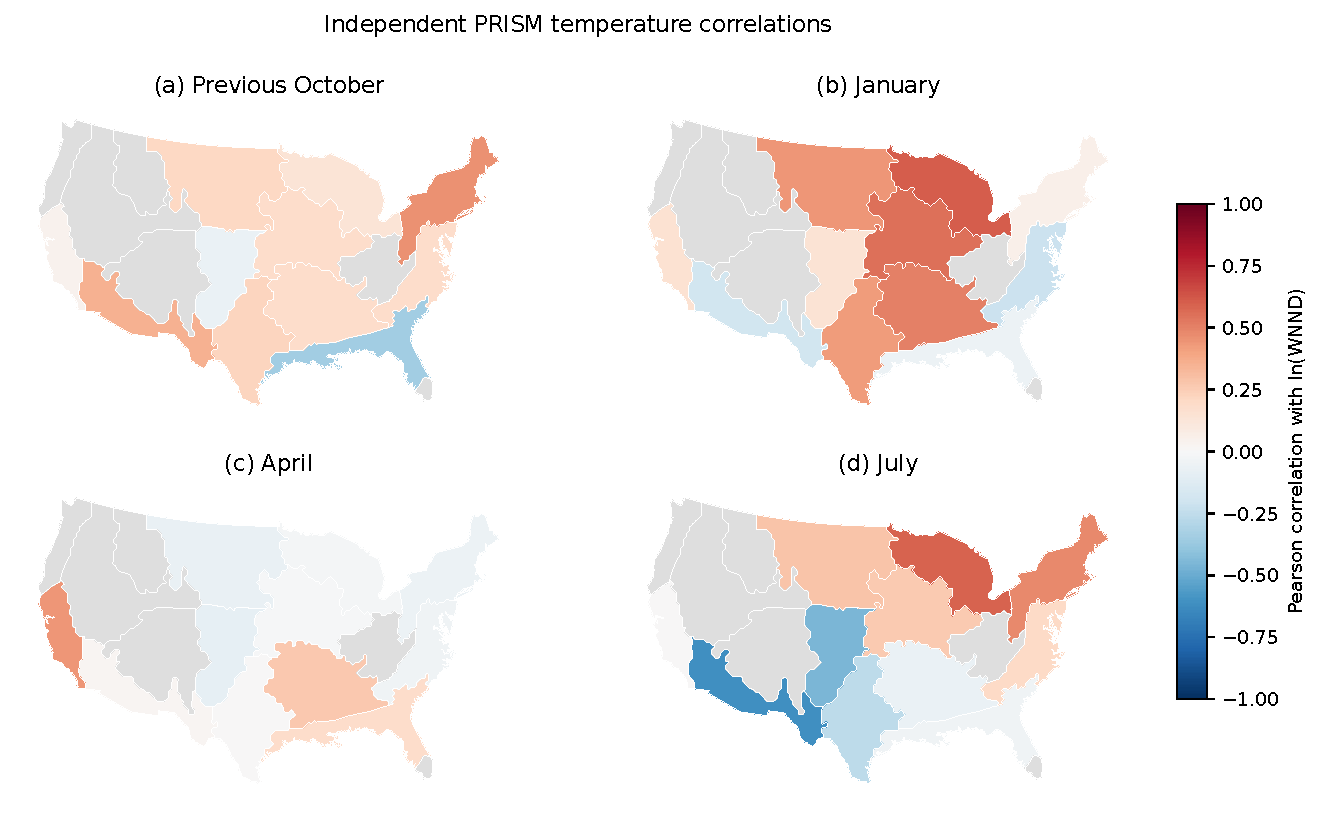
\includegraphics[width=\textwidth]{../figures/figure3.pdf}\caption{Independent Figure 3 reconstruction: the same calculation as Figure 2 for PRISM monthly mean temperature. The data are independently processed public grids, with no values extracted from published maps.}\end{figure}
\begin{figure}[H]\centering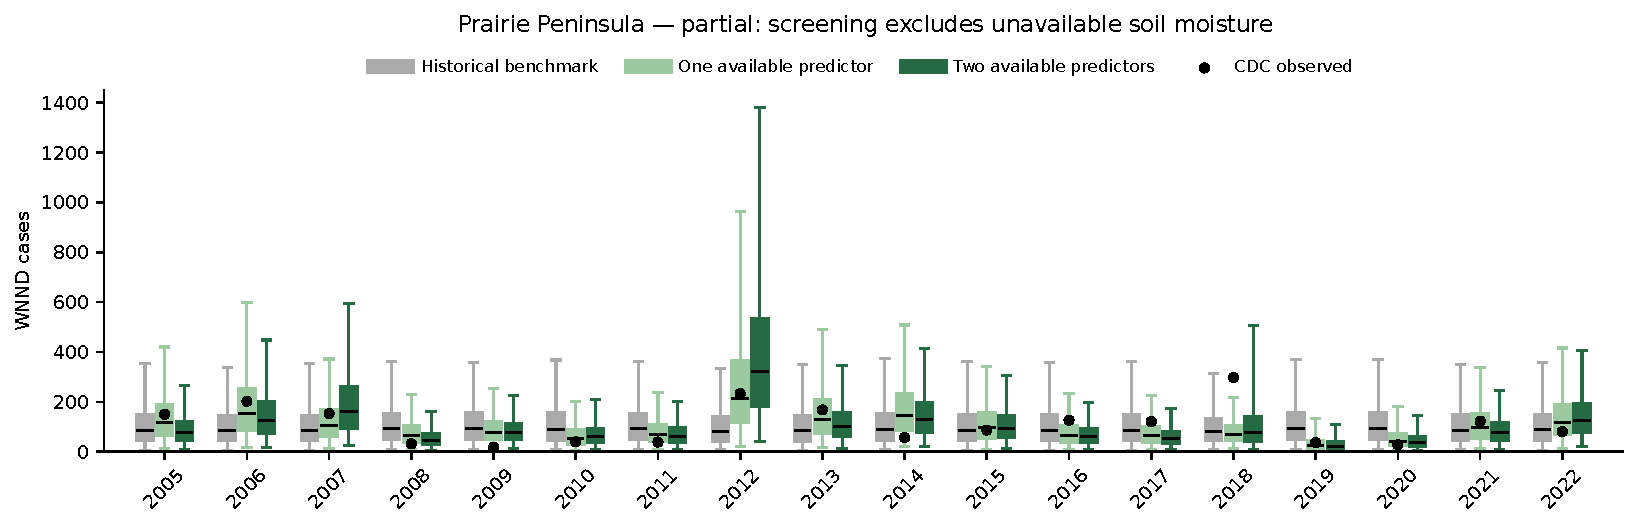
\includegraphics[width=\textwidth]{../figures/figure4.pdf}\caption{Partial Figure 4 reconstruction for Prairie Peninsula. Black points are CDC observations. Boxes show 25th, 50th and 75th predictive percentiles; whiskers span 2.5--97.5 percent. Grey is the historical benchmark. Green curves come from our restricted-candidate univariable and bivariable models because the published primary soil predictor is unavailable. They are independent calculations but do not complete reproduction of the published model.}\end{figure}
\begin{figure}[H]\centering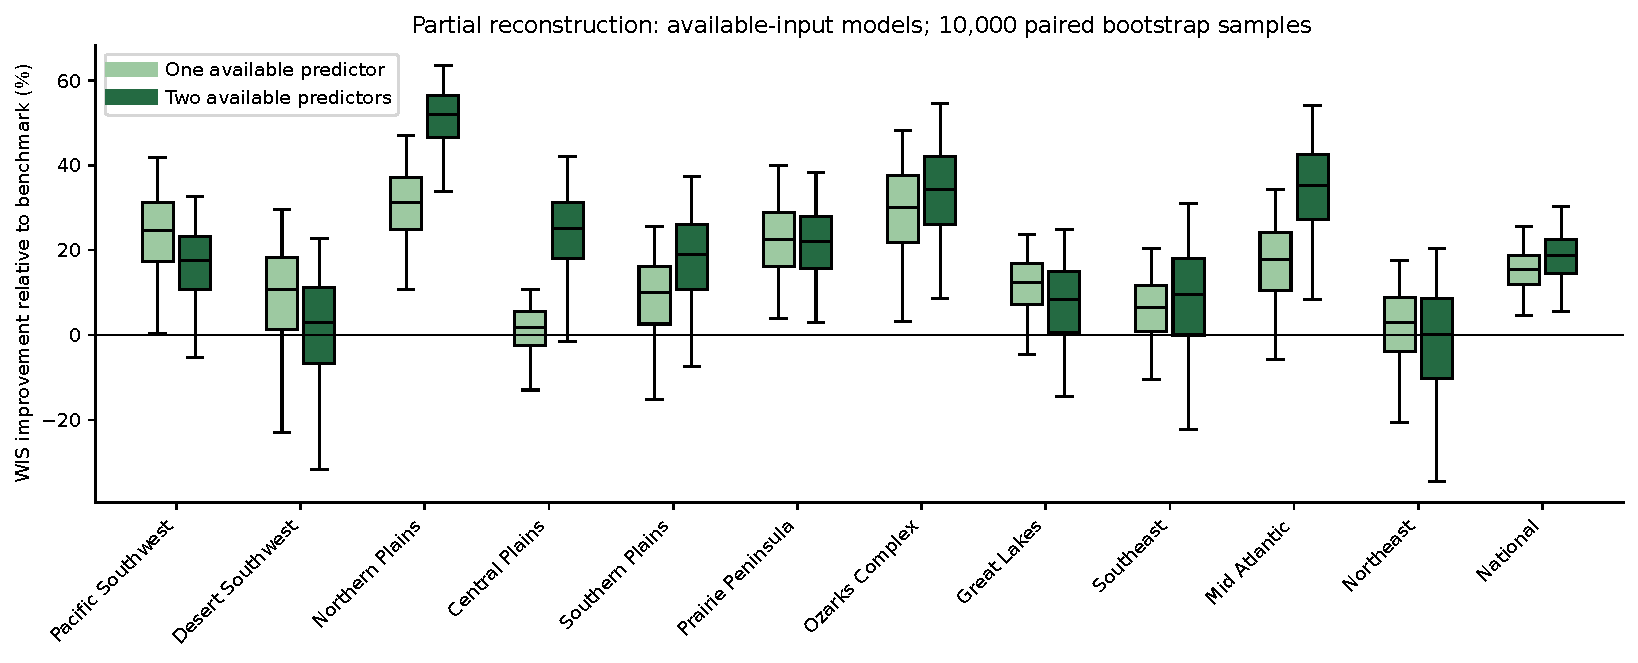
\includegraphics[width=\textwidth]{../figures/figure5.pdf}\caption{Partial Figure 5 reconstruction: relative WIS improvement for the independently selected available-input models. Boxes show bootstrap quartiles and whiskers span 95 percent intervals. National scores weight regional scores by case totals. The absent soil input limits comparability to the published full model.}\end{figure}
\subsection{Timing and magnitude of forecast errors}
\begin{table}[H]\centering\small\begin{tabular}{lrrrr}\toprule Region & Year & Observed & Forecast median & Signed error\\\midrule
Pacific Southwest & 2014 & 533 & 232 & -301 \\
Desert Southwest & 2021 & 1169 & 125 & -1044 \\
Northern Plains & 2013 & 157 & 96 & -61 \\
Central Plains & 2022 & 111 & 50 & -61 \\
Southern Plains & 2012 & 721 & 215 & -506 \\
Prairie Peninsula & 2018 & 298 & 77 & -221 \\
Ozarks Complex & 2017 & 153 & 65 & -88 \\
Great Lakes & 2012 & 328 & 86 & -242 \\
Southeast & 2011 & 61 & 244 & +183 \\
Mid Atlantic & 2012 & 134 & 55 & -79 \\
Northeast & 2018 & 196 & 65 & -131 \\
\bottomrule\end{tabular}\caption{Largest absolute median forecast error in each region for the available-input bivariable model. Positive values mean overprediction. Units are WNND cases. These errors are calculated from saved held-out forecasts.}\end{table}
The publication identifies the Desert Southwest 2021 outbreak as an influential failure case. Our 2021 observation is 1169 cases; the available-input bivariable median is 125, with a 95\% predictive interval [19, 505]. Exact published year-by-year predictions are not reported numerically in the text and were not digitized, so a numerical forecast-to-forecast error comparison is unavailable.
\section{Validation and limitations}
The likelihood agrees with an independent SciPy negative-binomial parameterization.
The WIS calculation agrees with its 23-quantile pinball-loss identity; a point
forecast equal to the observation scores exactly zero. Identical models remain
identical under the paired bootstrap. Training-fold standardization is isolated
from held-out covariates, and secondary predictor selection respects grouping.
Across 792 leave-one-year-out fits, the smallest importance effective sample size is 20067, largest Pareto $k$ is 0.457, and maximum mean Monte Carlo error is 0.018 posterior standard deviations. 0 fits fail the specified importance-sampling checks. The optimizer reports precision/status warnings for 0 proposals; these are retained in diagnostics. Since importance weights correct the proposal, these warnings alone do not establish a biased posterior, but poor weight diagnostics would fail the run.
The known-parameter experiment uses 240 synthetic counts with intercept 3, slopes 0.55 and -0.4, and NB shape 4. All four true values fall inside their 95\% posterior intervals. Over 24 repeated simulations, coverage is 91.7\%, 100.0\%, 100.0\%, 100.0\% for intercept, slope 1, slope 2, and shape. Four independent Metropolis chains give maximum R-hat 1.00, minimum bulk ESS 2680, and posterior mean differences below 0.027 posterior SD relative to importance sampling.
\begin{figure}[H]\centering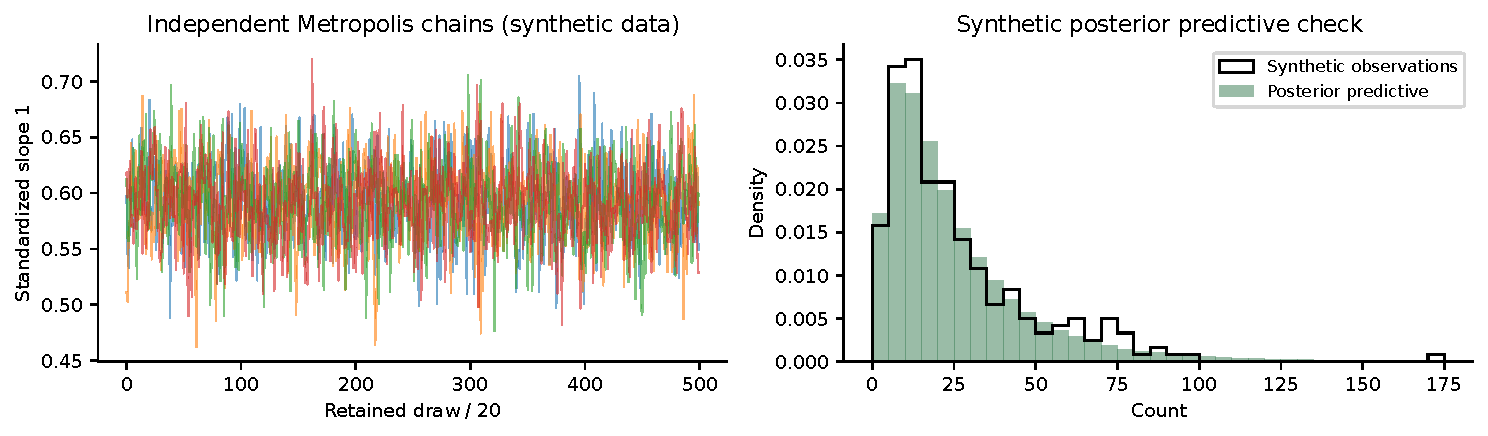
\includegraphics[width=\textwidth]{../figures/validation.pdf}\caption{Implementation validation using synthetic data, separate from manuscript reproduction. Left: four independent Metropolis traces for a standardized slope. Right: observed synthetic counts and posterior predictive distribution. Known parameters and intervals are saved in synthetic\_recovery.csv.}\end{figure}
We also compare four Metropolis chains with importance sampling for the observed fold with largest Pareto $k$ and for the Desert Southwest 2021 holdout using the published predictor pair. Across these two checks, maximum R-hat is 1.001, minimum bulk ESS is 2200, and the largest posterior mean difference is 0.026 posterior SD. All chain draws and check summaries are saved.
Full-data posterior predictive checks compare mean, variance, and maximum counts for each of three available-input models in all 11 regions. 0 of 99 observed summaries lie outside their 95\% posterior predictive intervals. These checks diagnose gross distributional mismatch; they are not independent tests of predictive skill. Held-out coverage, PIT values, and signed errors are saved separately.
The principal limitation is missing NLDAS soil moisture. Additional discrepancies
may arise from CDC revisions, spatial vintages, coastal assignments, grid-cell
approximation, PDSI monthly averaging, and inferred defaults. Full-record predictor
selection and climate weights allow information from held-out outcomes to enter
the workflow, and are therefore a limitation of the retrospective design itself.
No national result from the restricted-candidate run establishes or refutes the
paper's full-model improvement. The climate associations are predictive regressions
and do not isolate causal biological mechanisms.

The regional and county-level comparisons against the 2022 Forecasting Challenge
are not reproduced because external forecast outputs are excluded by the project
instructions. The county random-intercept extension is not implemented in this
regional pipeline. The main text's reference to logged county counts conflicts
with its supplement's count likelihood and also needs an explicit resolution
before that extension can be claimed reproduced.

\section{Build procedure and outcome}
The environment uses project-local Python 3.11.9 created by
\texttt{/usr/bin/python3.11 -m venv .venv}. All Python commands use the explicit
interpreter path. Exact installed dependencies are pinned in requirements.txt.
The clean procedure is:
\begin{verbatim}
bash scripts/setup.sh
bash scripts/rebuild.sh
\end{verbatim}
The first command recreates only .venv. The second downloads raw public inputs,
reconstructs processed data, fits models, validates numerical methods, creates all
plots, and compiles this report. For this delivered run, input downloads, processing,
fitting, validation, plotting, and PDF compilation were executed; build logs and
the final build outcome are stored in results. Cached raw files make repeat builds
faster. Fold caches are checked against a hash of inputs, predictor specifications,
random seeds, and modeling source before reuse. They are not independent input data.
The repository includes saved
processed inputs and computed outputs, so figures can also be regenerated offline.

TeX Live 2018 packages were checked with kpsewhich before writing the report:
article, geometry, amsmath, graphicx, booktabs, longtable, float, xcolor, caption,
subcaption, natbib, and hyperref. All were present. No system package was installed.
The unavailable siunitx package is not used; units are typeset with standard
mathematical roman text. The requested minimal-research and academic writing
guidance is linked and summarized in docs/guidance.md; no project-specific
vdv-damage content was used.

\section{Figure-by-figure record}
The machine-readable figure\_registry.csv contains one row per panel, source
documentation, input data, parameters, data command, plot command, and status.
For compactness, command keys below mean:
\begin{verbatim}
G: .venv/bin/python src/prepare.py geography
C: .venv/bin/python src/prepare.py climate
F: .venv/bin/python src/forecast.py
P: .venv/bin/python src/plot.py
\end{verbatim}
All numerical plots use saved independent output. R means independently reproduced,
P means partially reproduced, and N means not reproduced. R does not assert exact
agreement. Full source-specific assumptions are given above and in docs/method.md.
\small
\begin{longtable}{p{.09\textwidth}p{.24\textwidth}p{.32\textwidth}p{.21\textwidth}}
\toprule Panel & Quantity & Documentation / inputs / parameters & Status; data / plot command\\\midrule\endhead
1a & regional annual WNND mean & Section 2.2; Figure 1 caption; CDC; Census 2020; NEON Oct 2024; 2005-2022; zeros included & R; G / P; Descriptive observed-data reconstruction, not a model result; revised inputs and geography differ \\
1b & regional annual WNND median & Section 2.2; Figure 1 caption; CDC; Census 2020; NEON Oct 2024; 2005-2022; zeros included & R; G / P; Descriptive observed-data reconstruction, not a model result; revised inputs and geography differ \\
1c & county annual WNND mean & Section 2.2; Figure 1 caption; CDC; Census 2020; NEON Oct 2024; 2005-2022; zeros included & R; G / P; Descriptive observed-data reconstruction, not a model result; revised inputs and geography differ \\
1d & county annual WNND median & Section 2.2; Figure 1 caption; CDC; Census 2020; NEON Oct 2024; 2005-2022; zeros included & R; G / P; Descriptive observed-data reconstruction, not a model result; revised inputs and geography differ \\
2a & Pearson r: ln(WNND) vs previous October PDSI & Section 2.3; Figure 2 caption; CDC + gridMET; 18 years; log-total-case county weights & R; C, F / P; Independent correlations; numerical differences expected from input vintage and spatial processing \\
2b & Pearson r: ln(WNND) vs January PDSI & Section 2.3; Figure 2 caption; CDC + gridMET; 18 years; log-total-case county weights & R; C, F / P; Independent correlations; numerical differences expected from input vintage and spatial processing \\
2c & Pearson r: ln(WNND) vs April PDSI & Section 2.3; Figure 2 caption; CDC + gridMET; 18 years; log-total-case county weights & R; C, F / P; Independent correlations; numerical differences expected from input vintage and spatial processing \\
2d & Pearson r: ln(WNND) vs July PDSI & Section 2.3; Figure 2 caption; CDC + gridMET; 18 years; log-total-case county weights & R; C, F / P; Independent correlations; numerical differences expected from input vintage and spatial processing \\
3a & Pearson r: ln(WNND) vs previous October temperature & Section 2.3; Figure 3 caption; CDC + PRISM; 18 years; log-total-case county weights & R; C, F / P; Independent correlations; numerical differences expected from input vintage and spatial processing \\
3b & Pearson r: ln(WNND) vs January temperature & Section 2.3; Figure 3 caption; CDC + PRISM; 18 years; log-total-case county weights & R; C, F / P; Independent correlations; numerical differences expected from input vintage and spatial processing \\
3c & Pearson r: ln(WNND) vs April temperature & Section 2.3; Figure 3 caption; CDC + PRISM; 18 years; log-total-case county weights & R; C, F / P; Independent correlations; numerical differences expected from input vintage and spatial processing \\
3d & Pearson r: ln(WNND) vs July temperature & Section 2.3; Figure 3 caption; CDC + PRISM; 18 years; log-total-case county weights & R; C, F / P; Independent correlations; numerical differences expected from input vintage and spatial processing \\
4 & Prairie Peninsula annual probabilistic forecasts & Sections 2.4-2.5; Table 1; Text S2; CDC + available PRISM/gridMET; 17 training years; 23 quantiles; NB2 & P; F / P; Published primary soil moisture unavailable; generated restricted-candidate forecasts and benchmark \\
5 & Regional and national percent WIS improvement & Section 2.5; Text S1; Figure 5; Saved independent forecasts; Log1p WIS; 10000 paired bootstrap samples & P; F / P; National and regional restricted-candidate analysis omits soil moisture; published-pair scores saved where possible \\
S1 & Northeast monthly climate correlations & Section 2.3; Figure S1 caption; CDC; PRISM; gridMET; soil row missing; Oct(-1)-Jul; mask abs(r)<0.32 & P; F / P; Five of six climate rows independently computed; soil moisture row explicitly missing \\
S2 & Mid Atlantic monthly climate correlations & Section 2.3; Figure S2 caption; CDC; PRISM; gridMET; soil row missing; Oct(-1)-Jul; mask abs(r)<0.32 & P; F / P; Five of six climate rows independently computed; soil moisture row explicitly missing \\
S3 & Southeast monthly climate correlations & Section 2.3; Figure S3 caption; CDC; PRISM; gridMET; soil row missing; Oct(-1)-Jul; mask abs(r)<0.32 & P; F / P; Five of six climate rows independently computed; soil moisture row explicitly missing \\
S4 & Great Lakes monthly climate correlations & Section 2.3; Figure S4 caption; CDC; PRISM; gridMET; soil row missing; Oct(-1)-Jul; mask abs(r)<0.32 & P; F / P; Five of six climate rows independently computed; soil moisture row explicitly missing \\
S5 & Prairie Peninsula monthly climate correlations & Section 2.3; Figure S5 caption; CDC; PRISM; gridMET; soil row missing; Oct(-1)-Jul; mask abs(r)<0.32 & P; F / P; Five of six climate rows independently computed; soil moisture row explicitly missing \\
S6 & Ozarks Complex monthly climate correlations & Section 2.3; Figure S6 caption; CDC; PRISM; gridMET; soil row missing; Oct(-1)-Jul; mask abs(r)<0.32 & P; F / P; Five of six climate rows independently computed; soil moisture row explicitly missing \\
S7 & Northern Plains monthly climate correlations & Section 2.3; Figure S7 caption; CDC; PRISM; gridMET; soil row missing; Oct(-1)-Jul; mask abs(r)<0.32 & P; F / P; Five of six climate rows independently computed; soil moisture row explicitly missing \\
S8 & Central Plains monthly climate correlations & Section 2.3; Figure S8 caption; CDC; PRISM; gridMET; soil row missing; Oct(-1)-Jul; mask abs(r)<0.32 & P; F / P; Five of six climate rows independently computed; soil moisture row explicitly missing \\
S9 & Southern Plains monthly climate correlations & Section 2.3; Figure S9 caption; CDC; PRISM; gridMET; soil row missing; Oct(-1)-Jul; mask abs(r)<0.32 & P; F / P; Five of six climate rows independently computed; soil moisture row explicitly missing \\
S10 & Desert Southwest monthly climate correlations & Section 2.3; Figure S10 caption; CDC; PRISM; gridMET; soil row missing; Oct(-1)-Jul; mask abs(r)<0.32 & P; F / P; Five of six climate rows independently computed; soil moisture row explicitly missing \\
S11 & Pacific Southwest monthly climate correlations & Section 2.3; Figure S11 caption; CDC; PRISM; gridMET; soil row missing; Oct(-1)-Jul; mask abs(r)<0.32 & P; F / P; Five of six climate rows independently computed; soil moisture row explicitly missing \\
S12 & Northeast annual probabilistic forecasts & Table 1; Text S2; Figure S12 caption; CDC; PRISM/gridMET; 18 LOYO forecasts; NB2; 23 quantiles & P; F / P; Soil moisture required by published model unavailable; restricted-candidate curves and benchmark shown \\
S13 & Mid Atlantic annual probabilistic forecasts & Table 1; Text S2; Figure S13 caption; CDC; PRISM/gridMET; 18 LOYO forecasts; NB2; 23 quantiles & R; F / P; Both published predictor sets independently fitted; input/prior/numerical assumptions documented \\
S14 & Southeast annual probabilistic forecasts & Table 1; Text S2; Figure S14 caption; CDC; PRISM/gridMET; 18 LOYO forecasts; NB2; 23 quantiles & P; F / P; Soil moisture required by published model unavailable; restricted-candidate curves and benchmark shown \\
S15 & Great Lakes annual probabilistic forecasts & Table 1; Text S2; Figure S15 caption; CDC; PRISM/gridMET; 18 LOYO forecasts; NB2; 23 quantiles & P; F / P; Soil moisture required by published model unavailable; restricted-candidate curves and benchmark shown \\
S16 & Ozarks Complex annual probabilistic forecasts & Table 1; Text S2; Figure S16 caption; CDC; PRISM/gridMET; 18 LOYO forecasts; NB2; 23 quantiles & R; F / P; Both published predictor sets independently fitted; input/prior/numerical assumptions documented \\
S17 & Northern Plains annual probabilistic forecasts & Table 1; Text S2; Figure S17 caption; CDC; PRISM/gridMET; 18 LOYO forecasts; NB2; 23 quantiles & R; F / P; Both published predictor sets independently fitted; input/prior/numerical assumptions documented \\
S18 & Central Plains annual probabilistic forecasts & Table 1; Text S2; Figure S18 caption; CDC; PRISM/gridMET; 18 LOYO forecasts; NB2; 23 quantiles & R; F / P; Both published predictor sets independently fitted; input/prior/numerical assumptions documented \\
S19 & Southern Plains annual probabilistic forecasts & Table 1; Text S2; Figure S19 caption; CDC; PRISM/gridMET; 18 LOYO forecasts; NB2; 23 quantiles & P; F / P; Soil moisture required by published model unavailable; restricted-candidate curves and benchmark shown \\
S20 & Desert Southwest annual probabilistic forecasts & Table 1; Text S2; Figure S20 caption; CDC; PRISM/gridMET; 18 LOYO forecasts; NB2; 23 quantiles & R; F / P; Both published predictor sets independently fitted; input/prior/numerical assumptions documented \\
S21 & Pacific Southwest annual probabilistic forecasts & Table 1; Text S2; Figure S21 caption; CDC; PRISM/gridMET; 18 LOYO forecasts; NB2; 23 quantiles & P; F / P; Soil moisture required by published model unavailable; restricted-candidate curves and benchmark shown \\
S22 & Absolute WIS improvement & Section 2.5; Figure S22; Saved independent scores; 10000 paired bootstraps & P; F / P; Restricted-candidate model comparison \\
S23 & univariable PIT calibration histogram & Figure S23; Text S2; Saved posterior predictive draws; 198 held-out predictions; 10 equal bins; midpoint PIT & P; F / P; Restricted-candidate models; discrete PIT convention assumed \\
S24 & bivariable PIT calibration histogram & Figure S24; Text S2; Saved posterior predictive draws; 198 held-out predictions; 10 equal bins; midpoint PIT & P; F / P; Restricted-candidate models; discrete PIT convention assumed \\
Table S3 / Section 3.2 competition comparisons & County mixed-model and regional ensemble forecast skill & Section 2.6; Text S3; Table S3; Competition forecast submissions excluded; Not evaluated & N; not run; County extension not run; competition outputs excluded by independence constraint \\
\bottomrule\end{longtable}\normalsize\clearpage\appendix\section{Supplementary figure attempts}
\begin{figure}[H]\centering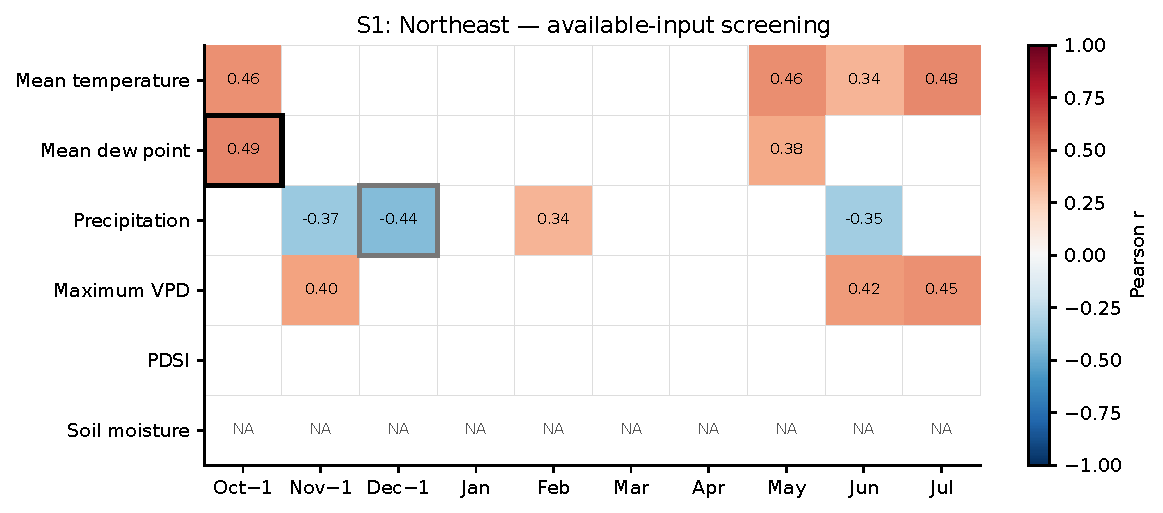
\includegraphics[width=\textwidth]{../figures/figureS1.pdf}\caption{Figure S1: Northeast monthly climate correlations. partially reproduced. Correlations use 18 years; white cells mask absolute r below 0.32, NA denotes unavailable soil moisture, and black/grey borders mark selected primary/secondary available predictors.}\end{figure}
\begin{figure}[H]\centering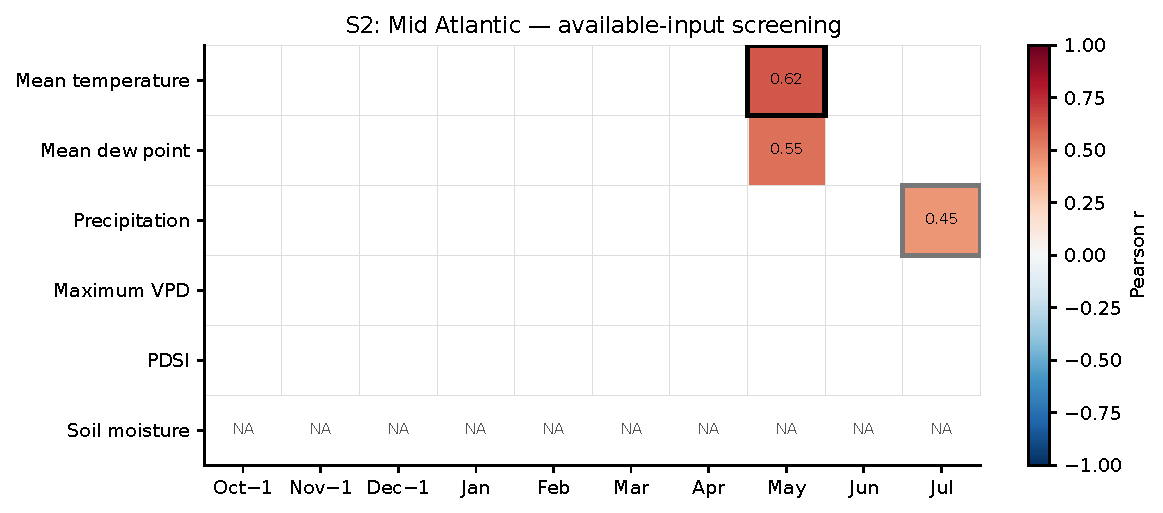
\includegraphics[width=\textwidth]{../figures/figureS2.pdf}\caption{Figure S2: Mid Atlantic monthly climate correlations. partially reproduced. Correlations use 18 years; white cells mask absolute r below 0.32, NA denotes unavailable soil moisture, and black/grey borders mark selected primary/secondary available predictors.}\end{figure}
\begin{figure}[H]\centering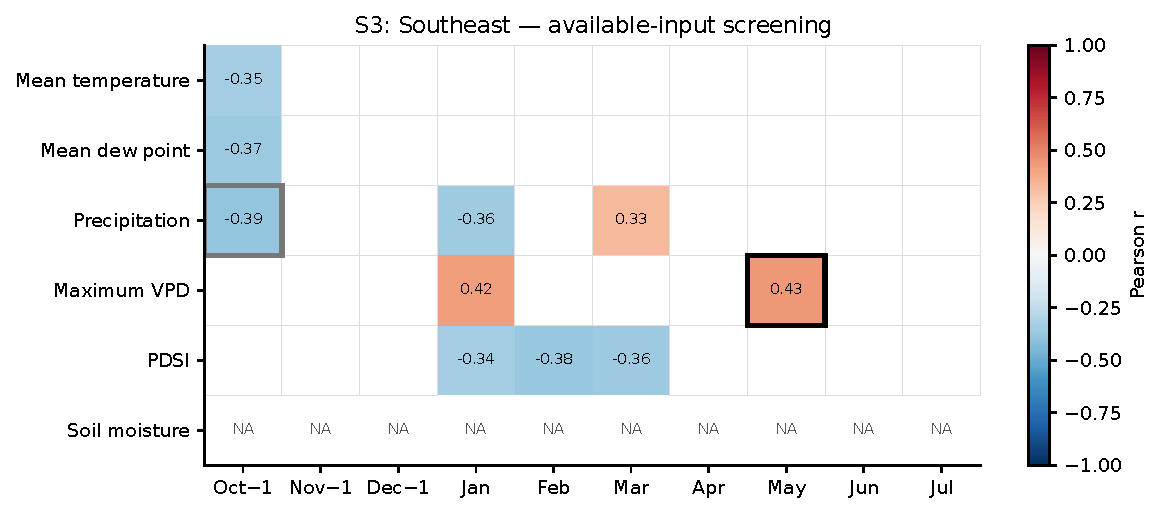
\includegraphics[width=\textwidth]{../figures/figureS3.pdf}\caption{Figure S3: Southeast monthly climate correlations. partially reproduced. Correlations use 18 years; white cells mask absolute r below 0.32, NA denotes unavailable soil moisture, and black/grey borders mark selected primary/secondary available predictors.}\end{figure}
\begin{figure}[H]\centering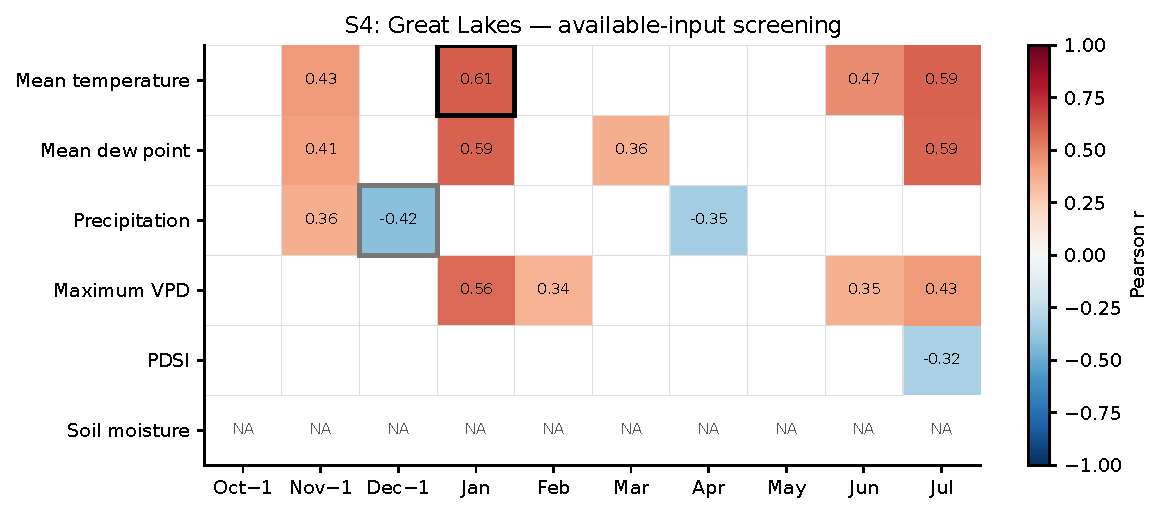
\includegraphics[width=\textwidth]{../figures/figureS4.pdf}\caption{Figure S4: Great Lakes monthly climate correlations. partially reproduced. Correlations use 18 years; white cells mask absolute r below 0.32, NA denotes unavailable soil moisture, and black/grey borders mark selected primary/secondary available predictors.}\end{figure}
\begin{figure}[H]\centering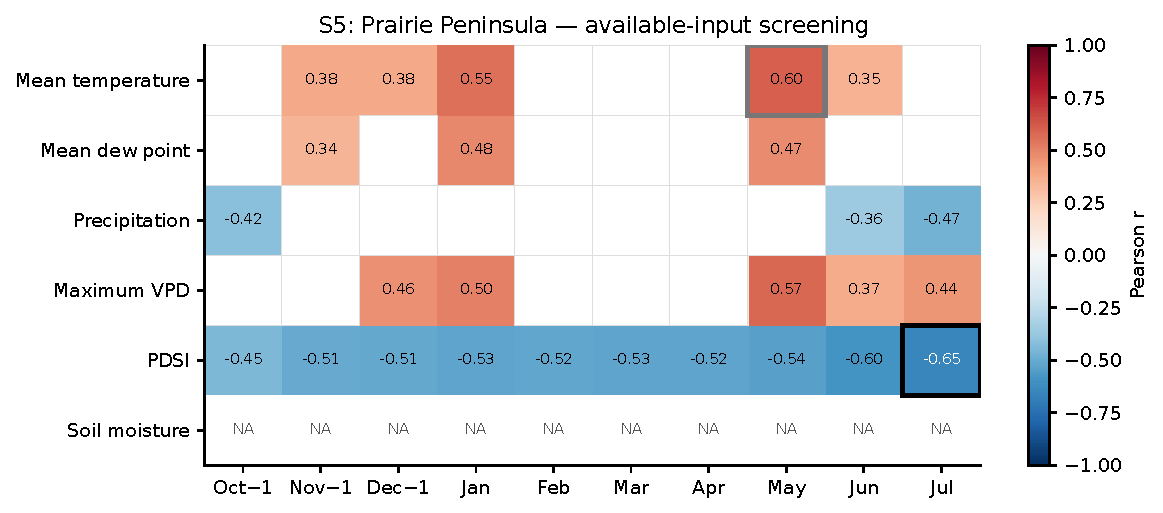
\includegraphics[width=\textwidth]{../figures/figureS5.pdf}\caption{Figure S5: Prairie Peninsula monthly climate correlations. partially reproduced. Correlations use 18 years; white cells mask absolute r below 0.32, NA denotes unavailable soil moisture, and black/grey borders mark selected primary/secondary available predictors.}\end{figure}
\begin{figure}[H]\centering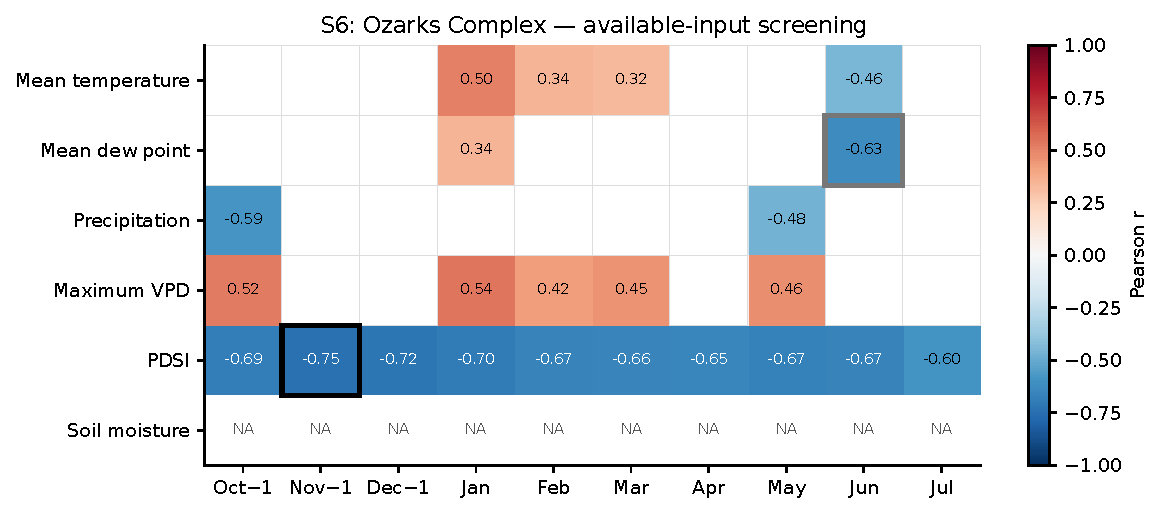
\includegraphics[width=\textwidth]{../figures/figureS6.pdf}\caption{Figure S6: Ozarks Complex monthly climate correlations. partially reproduced. Correlations use 18 years; white cells mask absolute r below 0.32, NA denotes unavailable soil moisture, and black/grey borders mark selected primary/secondary available predictors.}\end{figure}
\begin{figure}[H]\centering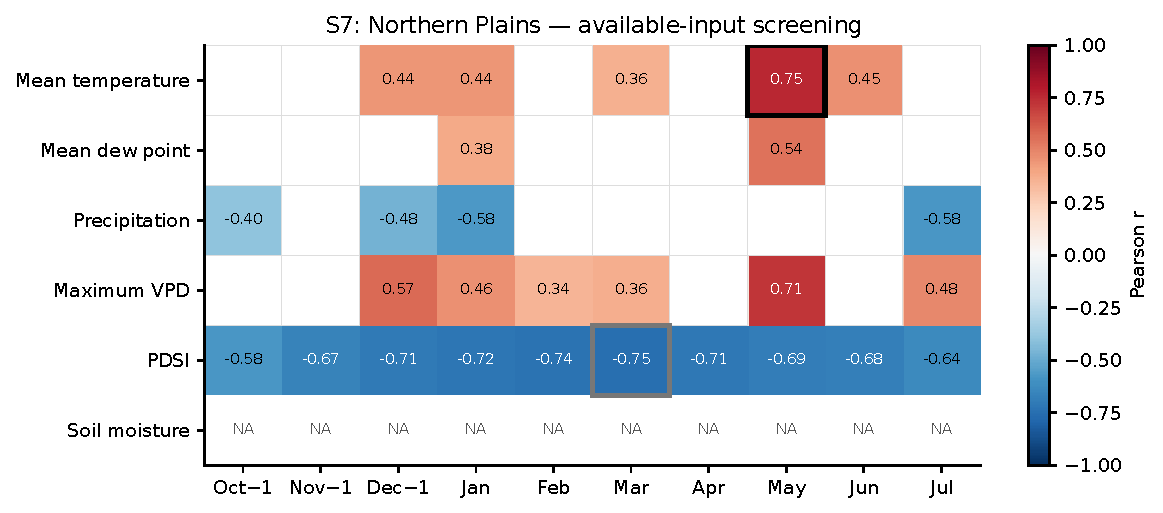
\includegraphics[width=\textwidth]{../figures/figureS7.pdf}\caption{Figure S7: Northern Plains monthly climate correlations. partially reproduced. Correlations use 18 years; white cells mask absolute r below 0.32, NA denotes unavailable soil moisture, and black/grey borders mark selected primary/secondary available predictors.}\end{figure}
\begin{figure}[H]\centering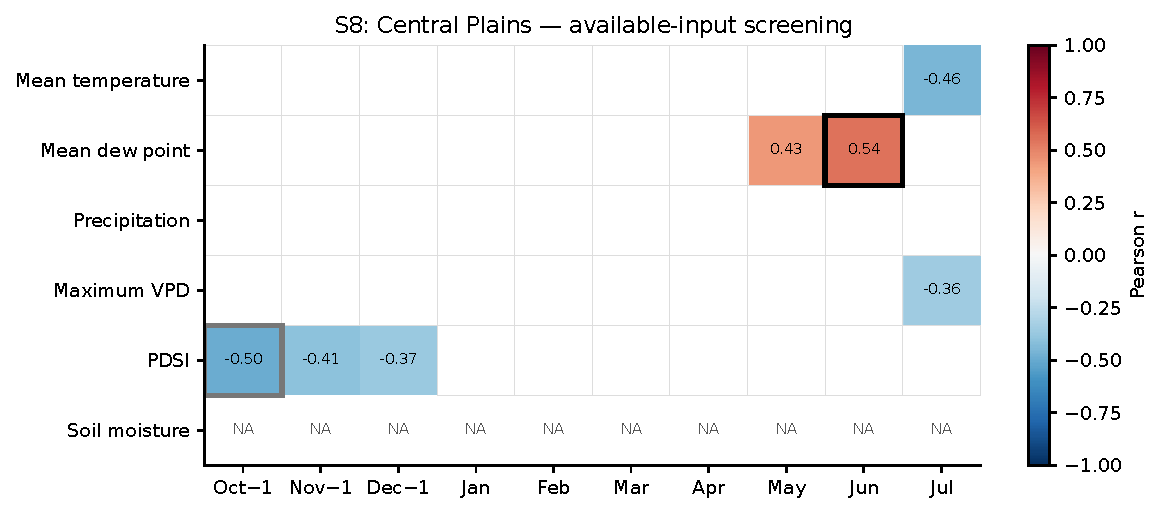
\includegraphics[width=\textwidth]{../figures/figureS8.pdf}\caption{Figure S8: Central Plains monthly climate correlations. partially reproduced. Correlations use 18 years; white cells mask absolute r below 0.32, NA denotes unavailable soil moisture, and black/grey borders mark selected primary/secondary available predictors.}\end{figure}
\begin{figure}[H]\centering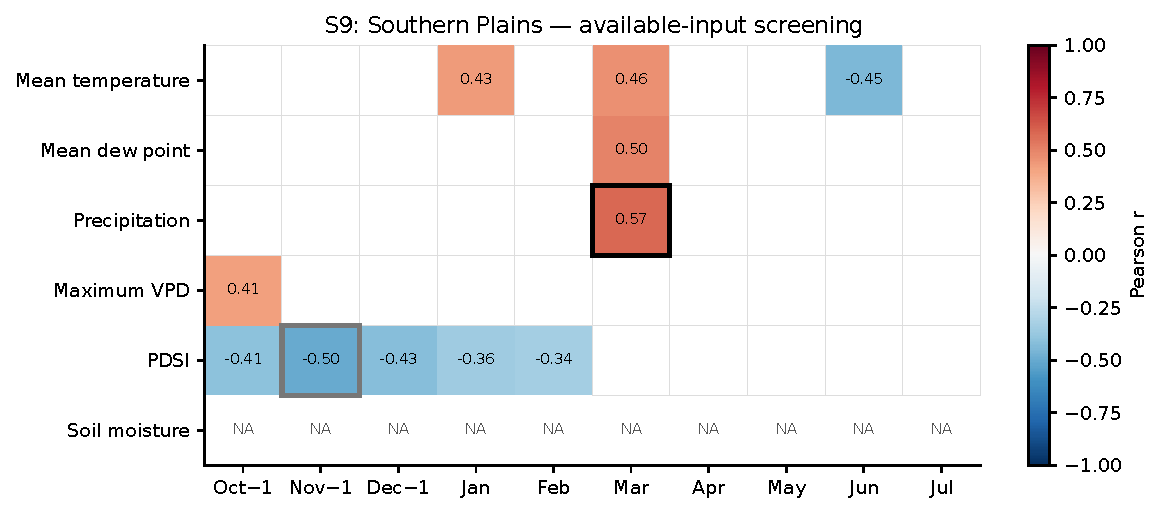
\includegraphics[width=\textwidth]{../figures/figureS9.pdf}\caption{Figure S9: Southern Plains monthly climate correlations. partially reproduced. Correlations use 18 years; white cells mask absolute r below 0.32, NA denotes unavailable soil moisture, and black/grey borders mark selected primary/secondary available predictors.}\end{figure}
\begin{figure}[H]\centering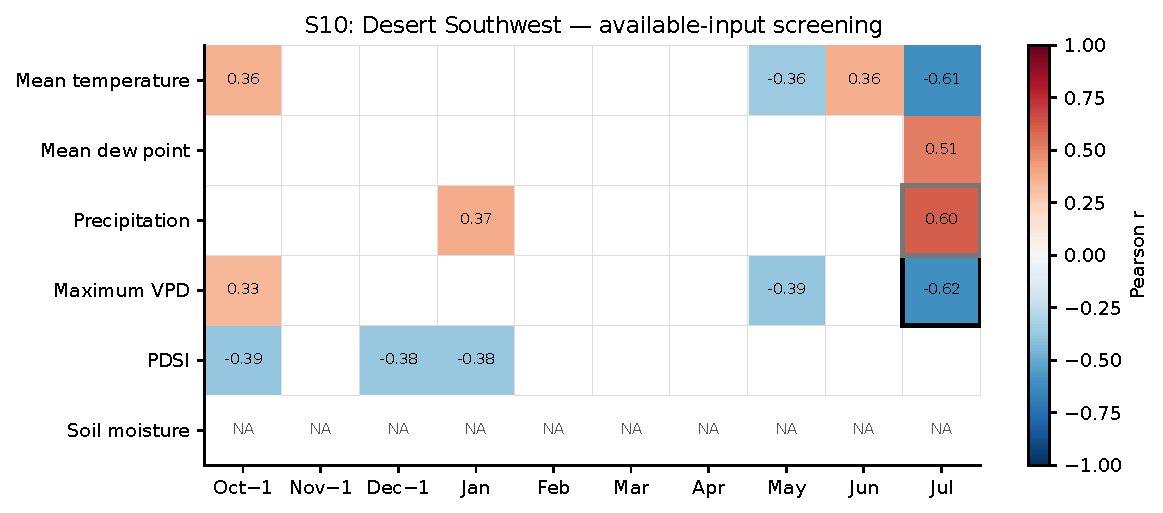
\includegraphics[width=\textwidth]{../figures/figureS10.pdf}\caption{Figure S10: Desert Southwest monthly climate correlations. partially reproduced. Correlations use 18 years; white cells mask absolute r below 0.32, NA denotes unavailable soil moisture, and black/grey borders mark selected primary/secondary available predictors.}\end{figure}
\begin{figure}[H]\centering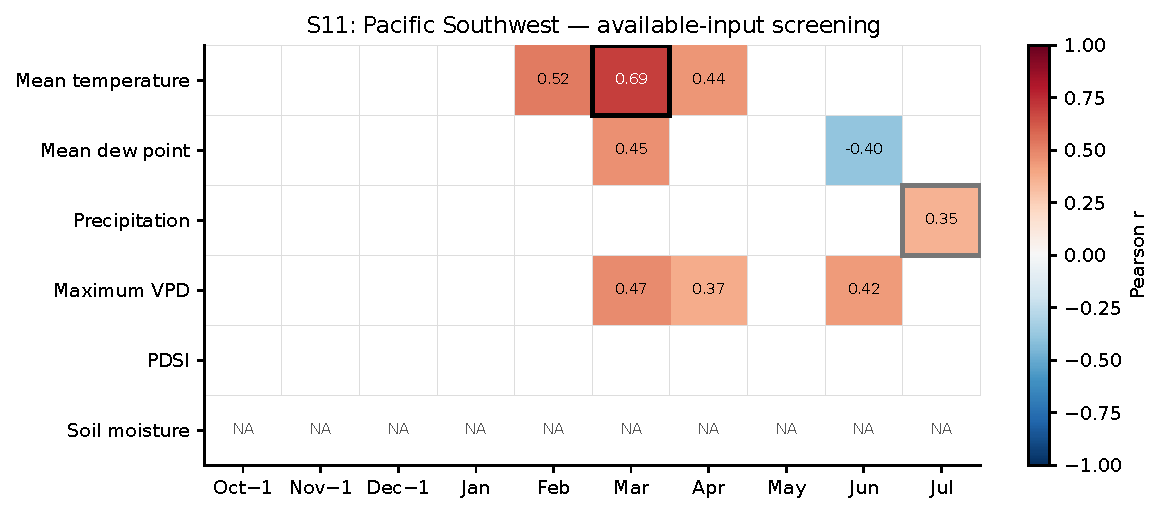
\includegraphics[width=\textwidth]{../figures/figureS11.pdf}\caption{Figure S11: Pacific Southwest monthly climate correlations. partially reproduced. Correlations use 18 years; white cells mask absolute r below 0.32, NA denotes unavailable soil moisture, and black/grey borders mark selected primary/secondary available predictors.}\end{figure}
\begin{figure}[H]\centering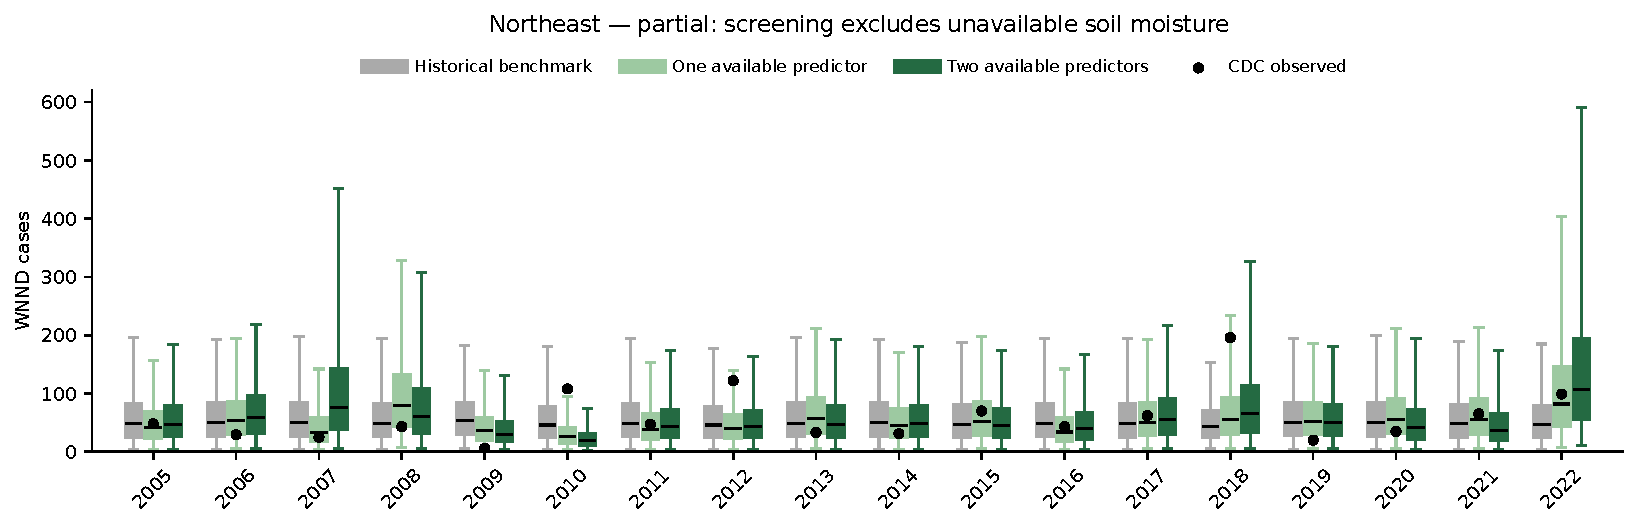
\includegraphics[width=\textwidth]{../figures/figureS12.pdf}\caption{Figure S12: Northeast annual probabilistic forecasts. partially reproduced. Box/whisker definitions match Figure 4. Titles distinguish published predictor sets from restricted-candidate models. Black points are CDC observations; all forecasts are independently generated.}\end{figure}
\begin{figure}[H]\centering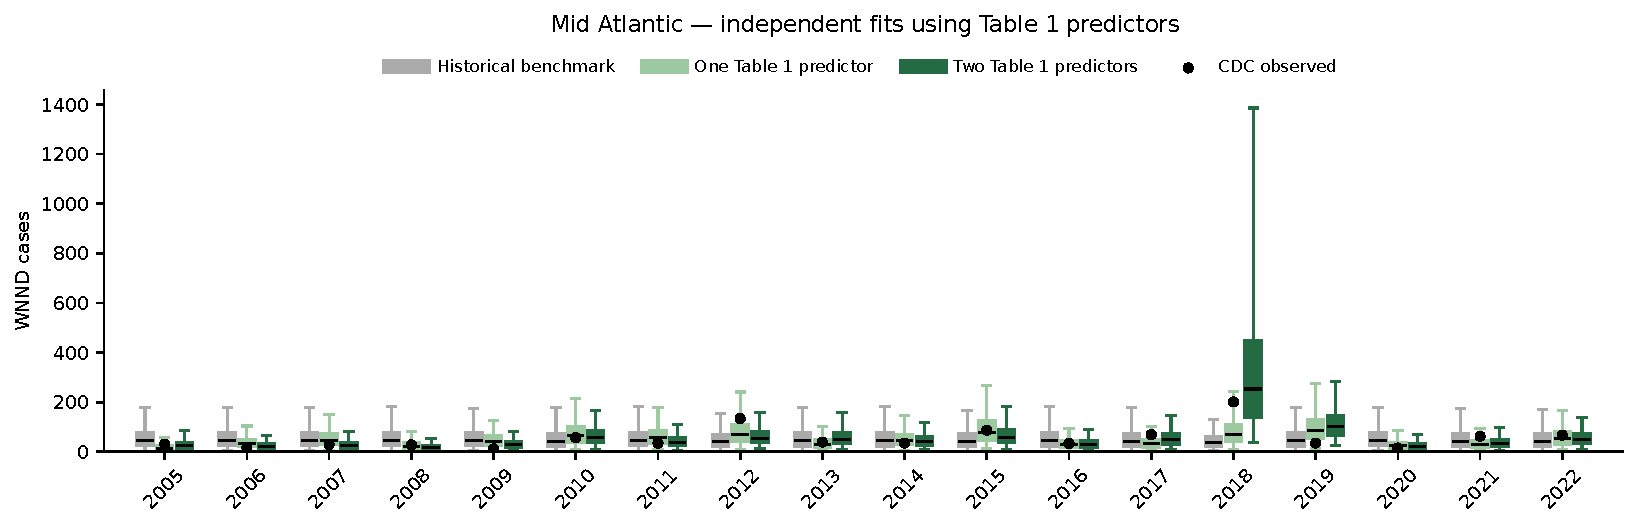
\includegraphics[width=\textwidth]{../figures/figureS13.pdf}\caption{Figure S13: Mid Atlantic annual probabilistic forecasts. independently reproduced. Box/whisker definitions match Figure 4. Titles distinguish published predictor sets from restricted-candidate models. Black points are CDC observations; all forecasts are independently generated.}\end{figure}
\clearpage
\begin{figure}[H]\centering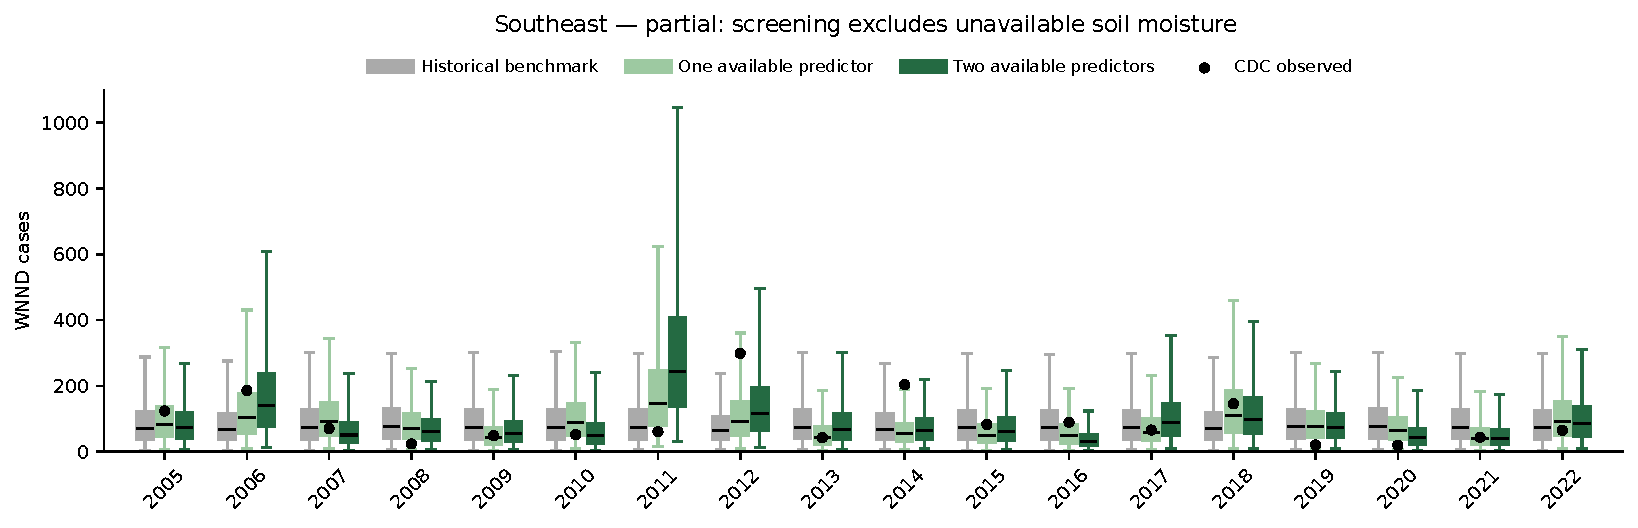
\includegraphics[width=\textwidth]{../figures/figureS14.pdf}\caption{Figure S14: Southeast annual probabilistic forecasts. partially reproduced. Box/whisker definitions match Figure 4. Titles distinguish published predictor sets from restricted-candidate models. Black points are CDC observations; all forecasts are independently generated.}\end{figure}
\begin{figure}[H]\centering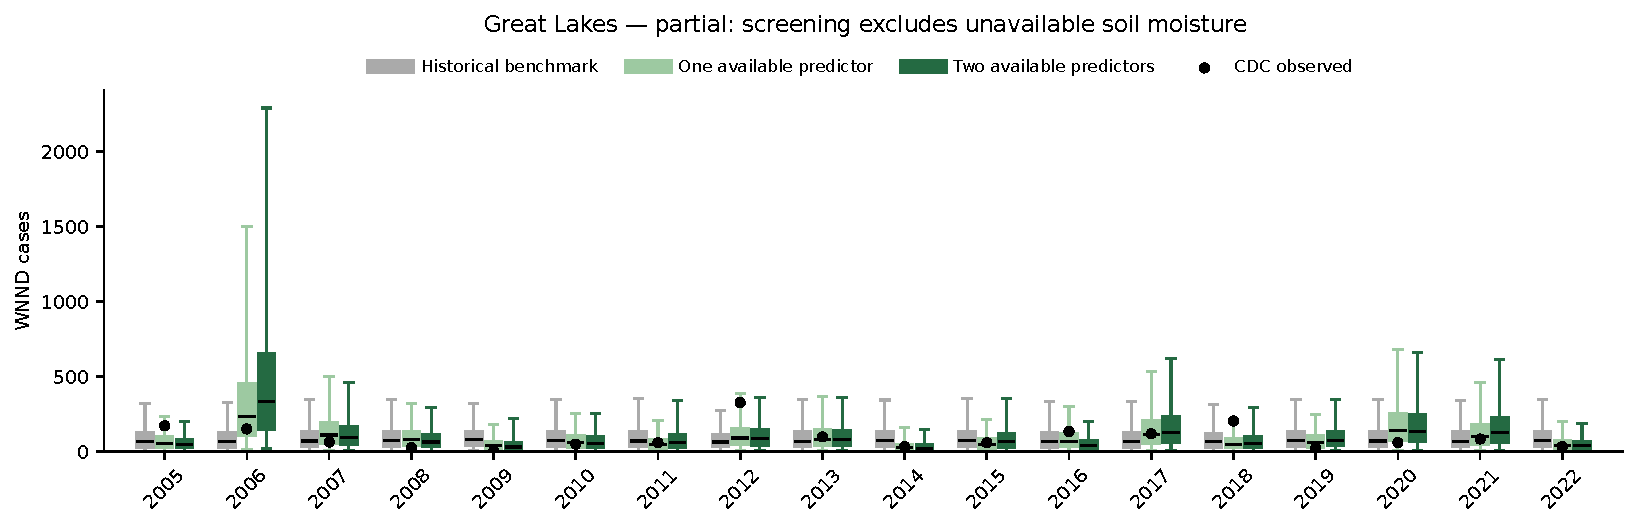
\includegraphics[width=\textwidth]{../figures/figureS15.pdf}\caption{Figure S15: Great Lakes annual probabilistic forecasts. partially reproduced. Box/whisker definitions match Figure 4. Titles distinguish published predictor sets from restricted-candidate models. Black points are CDC observations; all forecasts are independently generated.}\end{figure}
\clearpage
\begin{figure}[H]\centering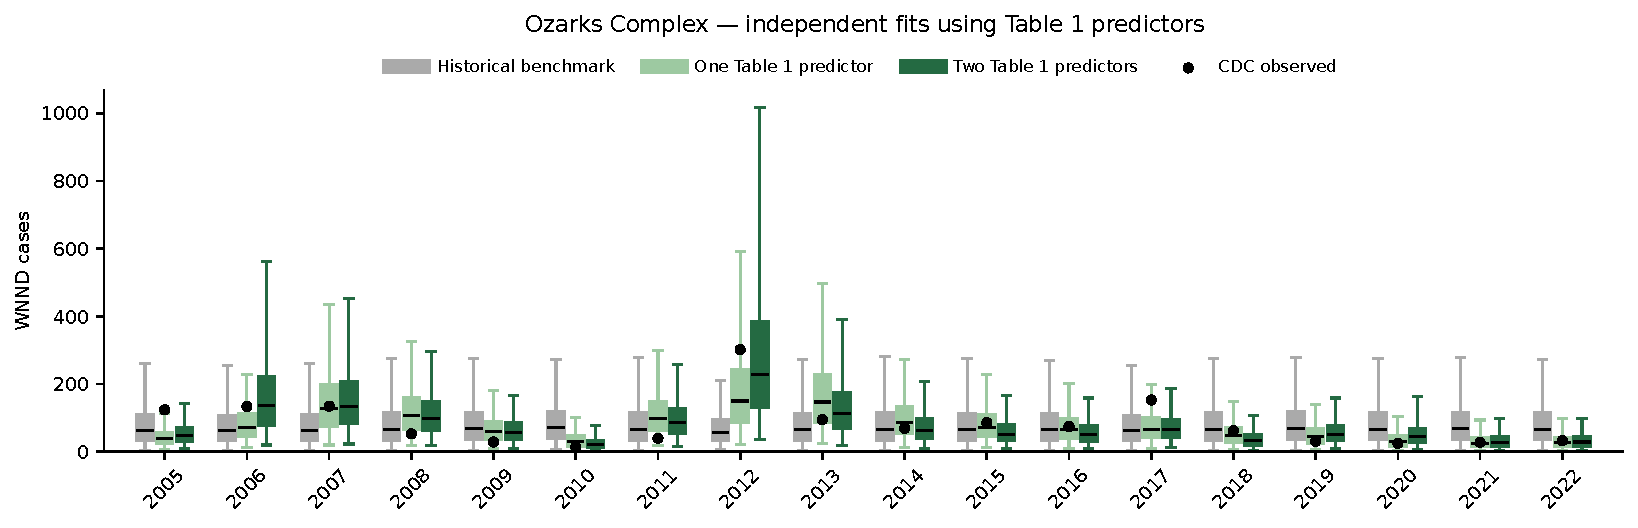
\includegraphics[width=\textwidth]{../figures/figureS16.pdf}\caption{Figure S16: Ozarks Complex annual probabilistic forecasts. independently reproduced. Box/whisker definitions match Figure 4. Titles distinguish published predictor sets from restricted-candidate models. Black points are CDC observations; all forecasts are independently generated.}\end{figure}
\begin{figure}[H]\centering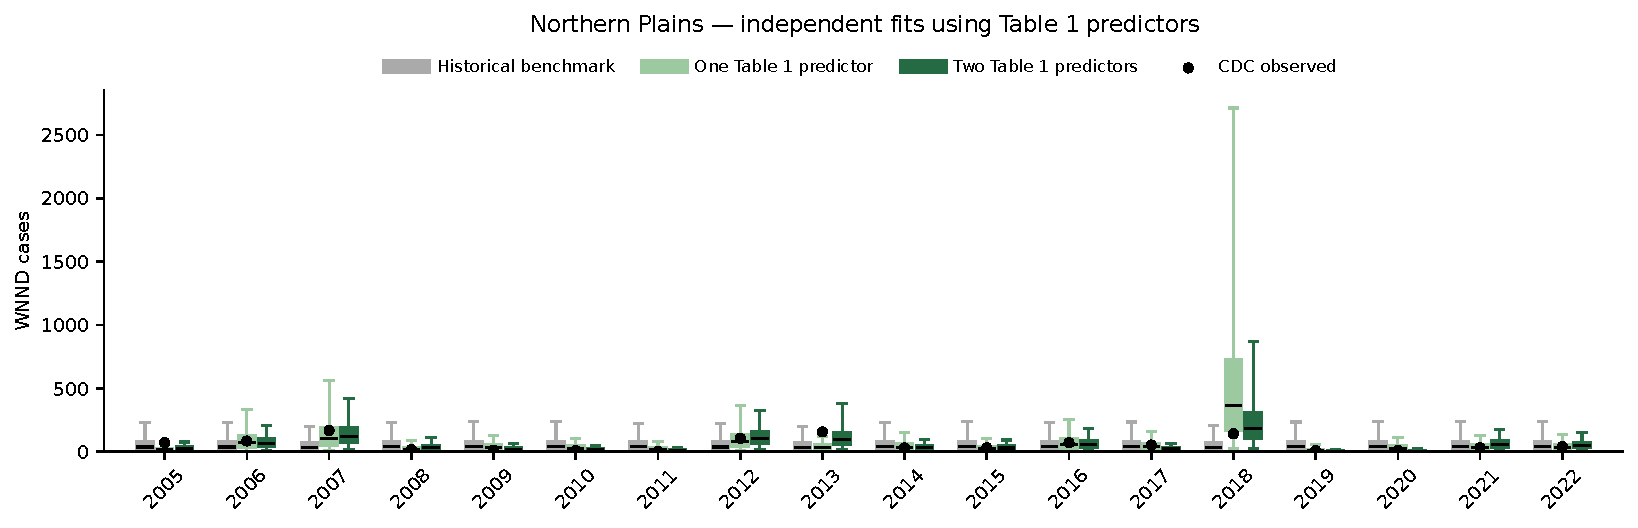
\includegraphics[width=\textwidth]{../figures/figureS17.pdf}\caption{Figure S17: Northern Plains annual probabilistic forecasts. independently reproduced. Box/whisker definitions match Figure 4. Titles distinguish published predictor sets from restricted-candidate models. Black points are CDC observations; all forecasts are independently generated.}\end{figure}
\clearpage
\begin{figure}[H]\centering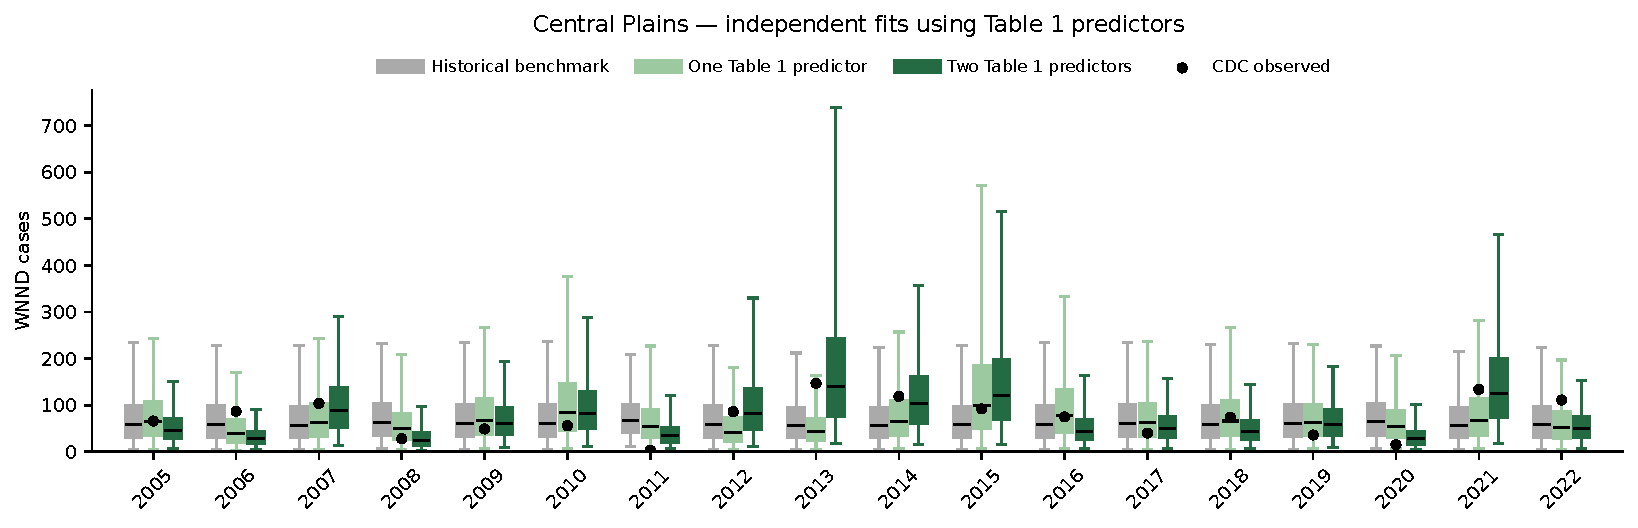
\includegraphics[width=\textwidth]{../figures/figureS18.pdf}\caption{Figure S18: Central Plains annual probabilistic forecasts. independently reproduced. Box/whisker definitions match Figure 4. Titles distinguish published predictor sets from restricted-candidate models. Black points are CDC observations; all forecasts are independently generated.}\end{figure}
\begin{figure}[H]\centering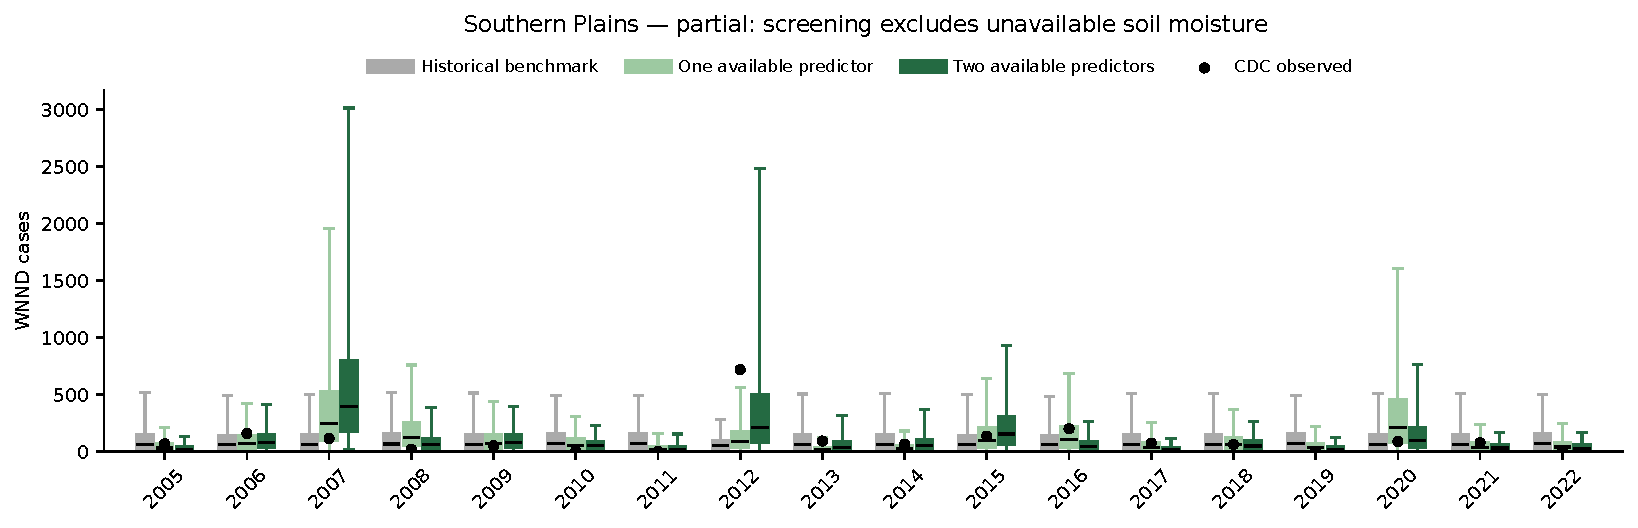
\includegraphics[width=\textwidth]{../figures/figureS19.pdf}\caption{Figure S19: Southern Plains annual probabilistic forecasts. partially reproduced. Box/whisker definitions match Figure 4. Titles distinguish published predictor sets from restricted-candidate models. Black points are CDC observations; all forecasts are independently generated.}\end{figure}
\clearpage
\begin{figure}[H]\centering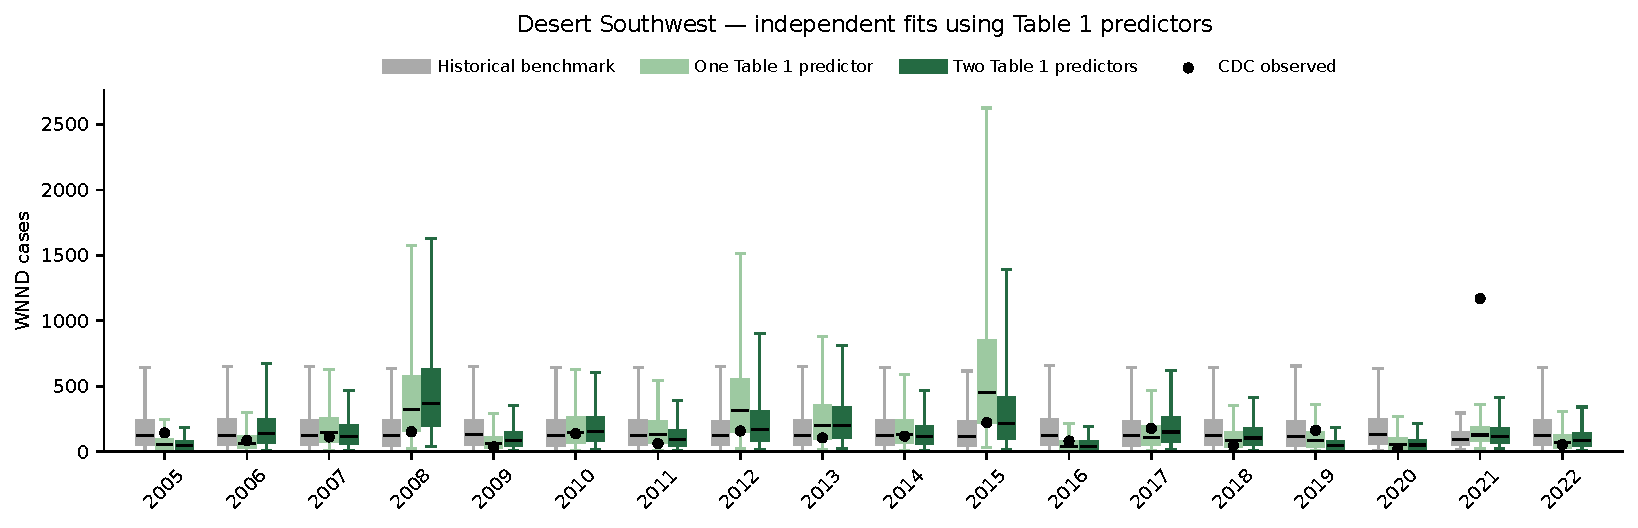
\includegraphics[width=\textwidth]{../figures/figureS20.pdf}\caption{Figure S20: Desert Southwest annual probabilistic forecasts. independently reproduced. Box/whisker definitions match Figure 4. Titles distinguish published predictor sets from restricted-candidate models. Black points are CDC observations; all forecasts are independently generated.}\end{figure}
\begin{figure}[H]\centering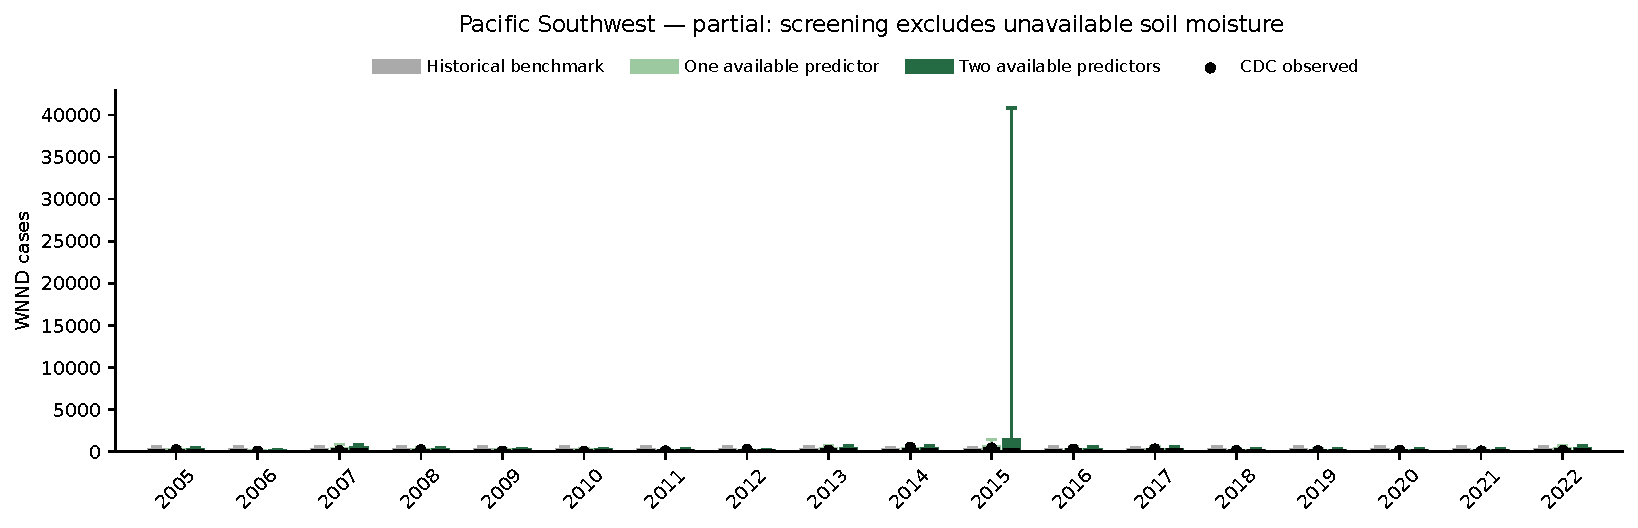
\includegraphics[width=\textwidth]{../figures/figureS21.pdf}\caption{Figure S21: Pacific Southwest annual probabilistic forecasts. partially reproduced. Box/whisker definitions match Figure 4. Titles distinguish published predictor sets from restricted-candidate models. Black points are CDC observations; all forecasts are independently generated.}\end{figure}
\clearpage
\begin{figure}[H]\centering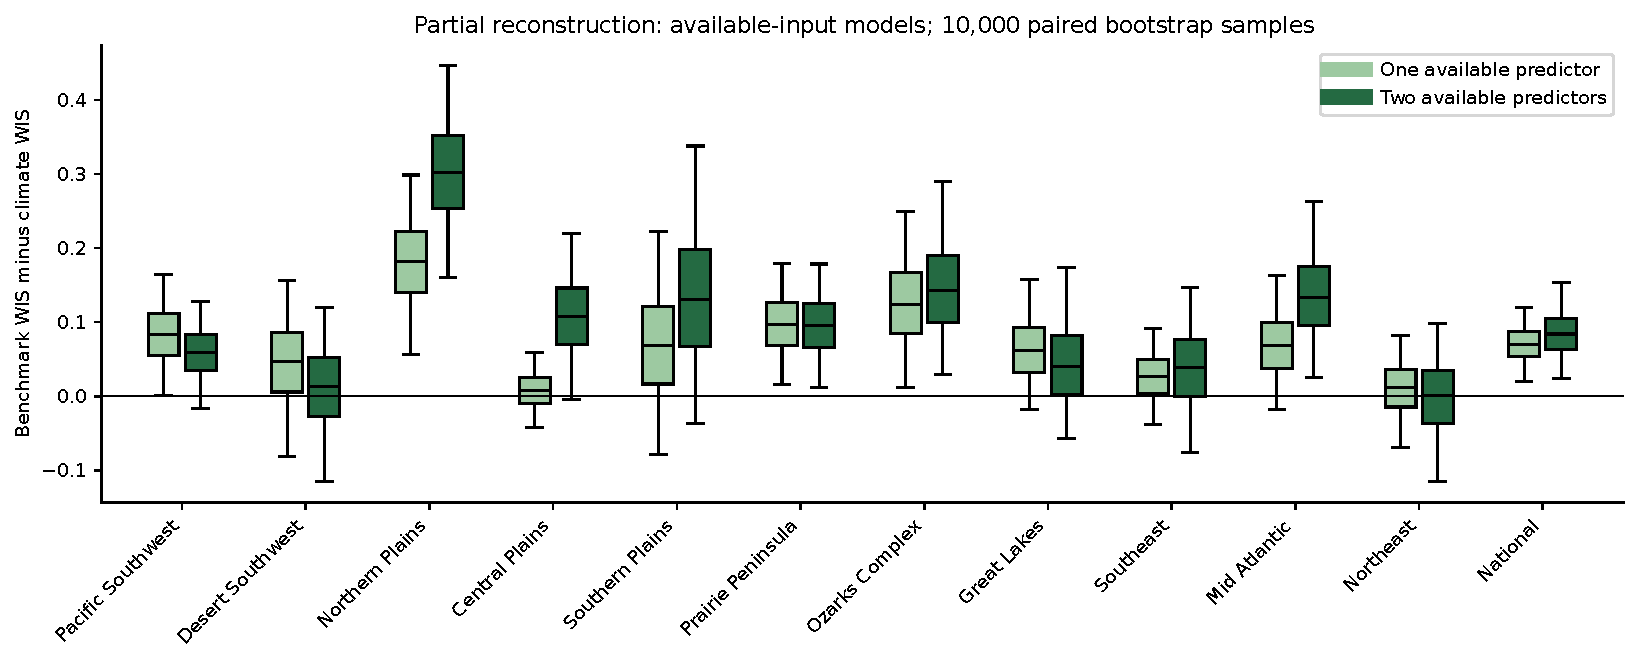
\includegraphics[width=\textwidth]{../figures/figureS22.pdf}\caption{Figure S22: Absolute WIS improvement. partially reproduced. Absolute log1p WIS improvement from 10,000 paired bootstrap samples; positive values favor climate information. Green shades distinguish one and two predictors.}\end{figure}
\begin{figure}[H]\centering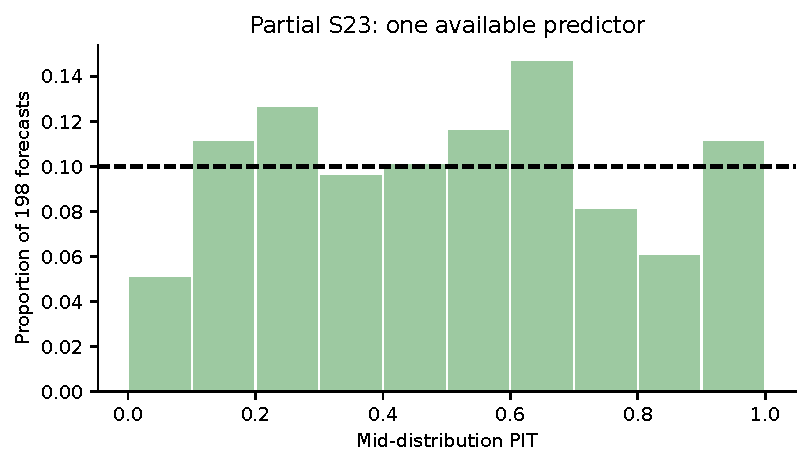
\includegraphics[width=\textwidth]{../figures/figureS23.pdf}\caption{Figure S23: univariable PIT calibration histogram. partially reproduced. Proportion of 198 held-out observations in each of ten midpoint-PIT bins. The dashed line is 0.10; nonuniformity indicates calibration departures under the stated discrete convention.}\end{figure}
\clearpage
\begin{figure}[H]\centering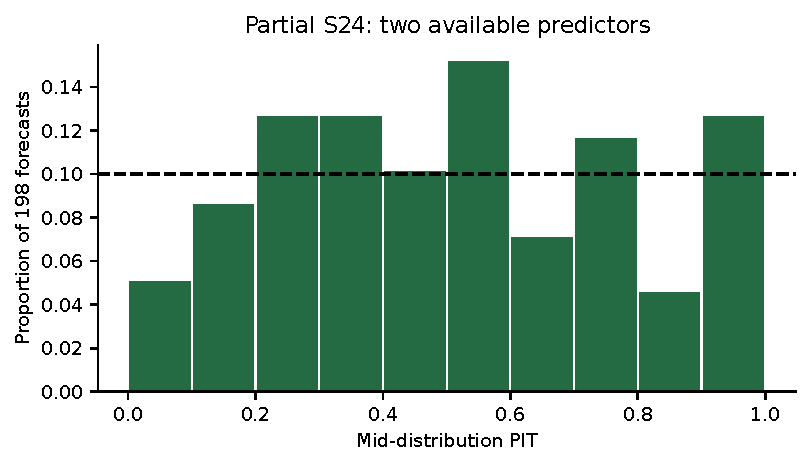
\includegraphics[width=\textwidth]{../figures/figureS24.pdf}\caption{Figure S24: bivariable PIT calibration histogram. partially reproduced. Proportion of 198 held-out observations in each of ten midpoint-PIT bins. The dashed line is 0.10; nonuniformity indicates calibration departures under the stated discrete convention.}\end{figure}
\begin{thebibliography}{9}
\bibitem[Harp et al.(2026)]{harp} Harp, R. D., et al. (2026).
A Regionally Determined Climate-Informed West Nile Virus Forecast Technique.
\emph{GeoHealth}, 10(2), e2025GH001657.
\url{https://doi.org/10.1029/2025GH001657}. Supporting Information S1, Texts S1--S3,
Figures S1--S24, Tables S1--S7.
\bibitem[Bracher et al.(2021)]{bracher} Bracher, J., Ray, E. L., Gneiting, T., and Reich, N. G. (2021).
Evaluating epidemic forecasts in an interval format. \emph{PLoS Computational Biology},
17, e1008618. \url{https://doi.org/10.1371/journal.pcbi.1008618}.
\bibitem[Stan Development Team(2026)]{rstanarm} Stan Development Team.
Prior distributions for rstanarm models. Accessed 8 October 2026.
\url{https://mc-stan.org/rstanarm/articles/priors.html}.
\bibitem[CDC(2026)]{cdc} Centers for Disease Control and Prevention.
Historic West Nile virus data. Finalized 16 September 2026; accessed 8 October 2026.
\url{https://www.cdc.gov/west-nile-virus/data-maps/historic-data.html}.
\bibitem[NEON(2024)]{neon} National Ecological Observatory Network.
Domain polygons, October 2024. \url{https://www.neonscience.org/field-sites/spatial-data-maps}.
\bibitem[Abatzoglou(2013)]{gridmet} Abatzoglou, J. T. (2013). Development of gridded
surface meteorological data for ecological applications and modelling.
\emph{International Journal of Climatology}, 33, 121--131.
\url{https://doi.org/10.1002/joc.3413}.
\end{thebibliography}
\end{document}
